% conductor_rho_line -- el conductor del orden de valores de caracteres de Sp(2m) en g_{1/q}.
% 16 de septiembre de 2026.  Carles Marin + Claude (asistente IA).
%
% REGLA DE REDACCION: resultados, no proceso.  Lo que se dice de un tercero es lo que esta en un
% articulo suyo, con localizador.  Lo medido va marcado como medido, con su cifra y su rango.
% Version 2: relato por preguntas, historia, figuras; incorpora la auditoria socratica del 16-sep.
%
% Compilar:  pdflatex conductor_rho_line (x2).  Figuras: python figuras.py
\documentclass[11pt,a4paper]{article}
\usepackage[T1]{fontenc}
\usepackage[utf8]{inputenc}
\usepackage{lmodern}
\usepackage[margin=2.6cm]{geometry}
\usepackage{amsmath,amssymb,amsthm}
\usepackage{graphicx}
\usepackage{booktabs}
\usepackage[dvipsnames,table]{xcolor}
\usepackage{float}
\usepackage[colorlinks=true,linkcolor=NavyBlue,citecolor=NavyBlue,urlcolor=NavyBlue,pagebackref=true,
  bookmarksnumbered=true,bookmarksopen=true]{hyperref}
\hypersetup{pdftitle={Where the character values of Sp(2m) at a torsion element fail to generate the ring of integers},
  pdfauthor={Carles Mar\'in}}
% cada referencia de la bibliografia enlaza a las paginas donde se cita
\renewcommand*{\backref}[1]{}
\renewcommand*{\backrefalt}[4]{{\footnotesize\textcolor{gray}{\ifcase #1 \or cited on page~#2.\else cited on
  pages~#2.\fi}}}
\usepackage{microtype}
\usepackage{needspace}
\renewcommand{\textfraction}{0.07}
\renewcommand{\topfraction}{0.92}
\renewcommand{\bottomfraction}{0.92}
\renewcommand{\floatpagefraction}{0.78}

\definecolor{azul}{HTML}{1F4E79}
\definecolor{fondoficha}{HTML}{EEF3F8}
\definecolor{filaclara}{HTML}{F2F6FA}

\newtheorem{theorem}{Theorem}
\newtheorem{proposition}[theorem]{Proposition}
\newtheorem{corollary}[theorem]{Corollary}
\newtheorem{lemma}[theorem]{Lemma}
\theoremstyle{definition}
\newtheorem{observation}[theorem]{Observation}
\newtheorem{question}[theorem]{Question}
\newtheorem{remark}[theorem]{Remark}

\newcommand{\Sp}{\mathrm{Sp}}
\newcommand{\ZZ}{\mathbb{Z}}
\newcommand{\QQ}{\mathbb{Q}}
\newcommand{\FF}{\mathbb{F}}
\newcommand{\cO}{\mathcal{O}}
\newcommand{\cf}{\mathfrak{f}}
\newcommand{\rad}{\mathfrak{r}}
\newcommand{\gr}{\operatorname{gr}}
\newcommand{\pregunta}[1]{\par\smallskip\noindent\emph{#1}\par\smallskip}
% pregunta de frontera al cierre de una seccion: discreta, sin cifras
\definecolor{azulpregunta}{HTML}{1F6FB2}
\newcommand{\frontera}[1]{\par\medskip\noindent{\small\color{azulpregunta}$\triangleright$\ \emph{#1}}\par}
% formula clave: enmarcada, numerada y enlazable
\newcommand{\marco}[1]{{\setlength{\fboxsep}{6pt}\setlength{\fboxrule}{0.6pt}%
  \fcolorbox{azul!45}{fondoficha}{$\displaystyle #1$}}}

\newsavebox{\fichabox}
\newenvironment{keybox}
  {\par\vspace{9pt}\begin{lrbox}{\fichabox}%
   \begin{minipage}{0.90\textwidth}\vspace{7pt}\setlength{\parskip}{3pt}}
  {\vspace{7pt}\end{minipage}\end{lrbox}%
   \par\needspace{\dimexpr\ht\fichabox+\dp\fichabox+12pt\relax}\noindent\hbox to \textwidth{\hfill
   \textcolor{azul}{\rule[-\dp\fichabox]{3.2pt}{\dimexpr\ht\fichabox+\dp\fichabox\relax}}%
   \colorbox{fondoficha}{\usebox{\fichabox}}\hfill}%
   \par\vspace{9pt}}

\title{\vspace{-1.4cm}\Large Where the character values of $\Sp(2m)$ at a torsion element\\
fail to generate the ring of integers}
\author{\normalsize Carles Mar\'in\thanks{Independent researcher, \texttt{karlesmarin@gmail.com}.
The author used Claude (Anthropic) as a research assistant, checked every statement, and takes full
responsibility for the content of this note.}}
\date{\normalsize 16 September 2026}

\begin{document}
\maketitle
\thispagestyle{empty}\enlargethispage{2pt}

\begin{abstract}
\noindent Let $g\in\Sp(2m)$ have eigenvalues $\xi_q^{\pm1},\dots,\xi_q^{\pm m}$, with $1\le m<q/2$. The values of
all characters of $\Sp(2m)$ at $g$ generate a subring $A$ of the ring of integers $\cO$ of $\QQ(\xi_q)^+$, which,
apart from known cases where it is $\ZZ$, is an order. We locate and describe its conductor. Write $h=2m$ and
$q=p^vq'$ with $p\nmid q'$. Every prime of the index $[\cO:A]$ divides $q$, and for $q'\notin\{1,2,3,4,6\}$ a prime
$p\mid q$ divides it if and only if $q'$ divides $h$, $h+1$ or $h+2$. At every prime the conductor is a power of
the radical. At such a $p$ with $\varphi(p^v)\ge2$, the first graded layer of $A$ has the dimension of the cyclic
module over $\FF_p[(\ZZ/q')^\times]$ generated by an explicit first-moment function $S$, and it decides whether that
power is $1$ and, when it is $2$, both lengths and whether the local ring is Gorenstein. For $p$ odd and
$q'\notin\{1,2,3,4,6\}$, the stable segments give $S$ two shapes: Stickelberger's sawtooth when
$m\equiv0,-1\pmod{q'}$, and that sawtooth shifted by half a period when $2m+1=Nq'$ or when $q'$ is even and
$m\equiv q'/2,q'/2-1\pmod{q'}$. On the sawtooth families and on the half-period ones with $q'$ even, a half-period
identity and a doubling lemma put the two on one lattice, and Sinnott's index formula computes the $p$-part of the
maximal minors of the moment matrix: the conductor at $p$ is the radical exactly when $p$ does not divide
$h^-(\QQ(\zeta_{q'}))$, and a simple divisor of $h^-$ gives the square of the radical at $p$ and a Gorenstein local ring. When
instead $2m+1=Nq'$ and $p\nmid N\,h^-$, the first layer, both lengths and the Cohen--Macaulay type are read off the
subgroup generated by $2$ in $(\ZZ/q')^\times$. Whenever that first layer, of dimension $w$, is more than half full,
the index at $p$ is settled: $v_p([\cO:A])=2d-1-w$, with $d=\varphi(q')/2$ the dimension of the residue ring. The answers bring together
Dedekind's conductor, Kummer's link between Bernoulli numbers and class numbers, and the combinatorics of musical
scales.
\end{abstract}

\medskip
\noindent\textbf{Keywords:} character values; orders in cyclotomic fields; conductor; Stickelberger
ideal; Gorenstein ring; relative class number.

% ==============================================================================================
\section{What this note is about}\label{sec:intro}

A character of a compact Lie group, evaluated at an element of finite order, is an algebraic integer.
Take all characters at once, at one element, and they generate a ring. For the element
$g=g_{1/q}\in\Sp(2m)$ with eigenvalues $\xi_q^{\pm j}$, $1\le j\le m$, that ring sits inside the ring of
integers $\cO=\ZZ[\xi_q+\xi_q^{-1}]$ of the real cyclotomic field. Two questions follow, one inside the
other:

\pregunta{Do the character values generate the ring of integers? And where they do not, what exactly is
missing?}

\noindent Both questions are older than the ring. In 1877, counting ideal classes in orders of a number field,
Dedekind attached to each order the largest ideal of the maximal order that it contains, its \emph{Führer}, or
conductor \cite{Ded77}. A year later he showed that above a prime $p$ not dividing the index $[\cO:\ZZ[\alpha]]$ the
primes of $\cO$ can be read off the factorisation of the minimal polynomial of $\alpha$ modulo $p$ \cite{Ded78}.
Which primes divide the index, and what the conductor looks like at each of them, have been the first things to
ask about an order ever since. What changes here is who chooses the generators: not one number $\alpha$, but every
irreducible character of $\Sp(2m)$, evaluated at once at $g$.

\noindent The first question has a clean answer, and the answer to the second turns out to be written in
three older languages: the combinatorics of musical scales, the length formalism of one-dimensional rings,
and the arithmetic of Bernoulli numbers. The note is organised as a sequence of questions, each one raised
by the answer to the previous one. Figure~\ref{fig:estructura} draws that thread, and the table lists the answers.

\begin{figure}[htbp]
\centering
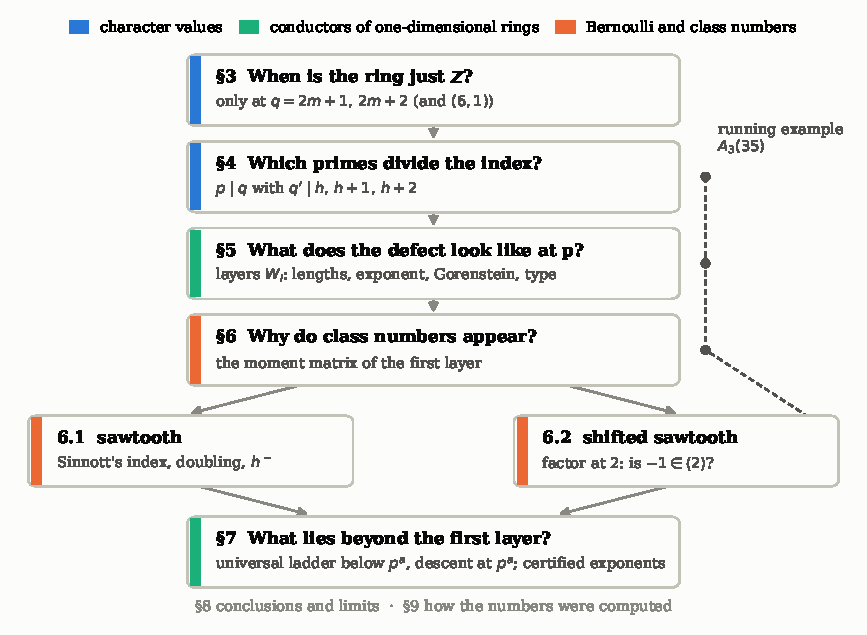
\includegraphics[width=0.94\textwidth]{fig_estructura.pdf}
\caption{The thread of the note. Each section answers the question left by the one above it; at \S\ref{sec:clase} the
two kinds of stable segment split the answer in two. The colour of each box marks which of the three lines of
\S\ref{sec:historia} it draws on, and the dashed line follows the running example $A_3(35)$.}
\label{fig:estructura}
\end{figure}

\medskip
\begin{center}\small
\rowcolors{2}{filaclara}{white}
\begin{tabular}{p{0.44\textwidth}p{0.47\textwidth}}
\toprule
question & answer \\
\midrule
When is the ring just $\ZZ$? (\S\ref{sec:set}) & exactly at the integer points of an earlier note: Proposition~\ref{prop:AZ} \\
Which primes divide the index? (\S\ref{sec:sop}) & only primes of $q$; and, for $q'\notin\{1,2,3,4,6\}$, $p\mid[\cO:A]$ iff the prime-to-$p$ part $q'$ of the order of $g$ divides $h$, $h+1$ or $h+2$: Theorem~\ref{thm:sop}, Figure~\ref{fig:paisaje} \\
What does the defect look like at one prime? (\S\ref{sec:loc}) & a single residue field $\FF_p$, a first layer measured by a cyclic module, lengths as sums of layer defects, a Gorenstein criterion and the Cohen--Macaulay type: Theorem~\ref{thm:loc}, Propositions~\ref{prop:cert}--\ref{prop:tipo} \\
Why do class numbers appear? (\S\ref{sec:clase}) & the maximal minors of the moment matrix are Sinnott's index (up to a power of $2$ when $q'\equiv2\pmod4$), so $h^-$ decides whether the first layer is full; for $2m+1=Nq'$ and $p\nmid N\,h^-$ the subgroup $\langle2\rangle$ decides it: Proposition~\ref{prop:sinnott}, Lemma~\ref{lem:dobla}, Theorem~\ref{thm:hminus}, Corollaries~\ref{cor:simple}, \ref{cor:dos}, Figures~\ref{fig:sierra}--\ref{fig:stickel} \\
What lies beyond the first layer? (\S\ref{sec:capas}) & a universal ladder below $p^{v_p(N)}$, descent to a smaller order at $p^{v_p(N)}$, exponents certified by semigroups, and a question on what lies beyond: Propositions~\ref{prop:escalera}, \ref{prop:descenso}, Corollary~\ref{cor:semigrupo}, Figure~\ref{fig:perfil} \\
What is proved, and where does it stop? (\S\ref{sec:open}) & what is ours, what rests on others, what was only measured, and what is not covered \\
\bottomrule
\end{tabular}
\end{center}


\noindent\textbf{A running example.} Take $m=3$ and $q=35$, so $A=A_3(35)$ has rank $\varphi(35)/2=12$ and $h=6$. At
$p=7$, $q'=5$ divides none of $6,7,8$; at $p=5$, $q'=7=h+1$. So only $5$ divides the index, and the example is
followed through \S\S\ref{sec:sop}--\ref{sec:clase} until $[\cO:A]=5^3$ and $\cf\,\cO_5=\rad^2$ come out by hand.

\medskip
\begin{center}\small
\rowcolors{2}{filaclara}{white}
\begin{tabular}{llp{0.62\textwidth}}
\toprule
symbol & & meaning \\
\midrule
$q$, $\xi$, $K$, $\cO$ & & order of $g$; $\xi=\xi_q$; $K=\QQ(\xi)^+$; $\cO=\ZZ[\xi+\xi^{-1}]$ \\
$m$, $h$ & & rank; $h=2m$, the Coxeter number of $C_m$ \\
$A$, $\cf$ & & the order~\eqref{eq:A}; its conductor $(A:\cO)$ \\
$p$, $v$, $q'$, $E$ & & a prime; $q=p^vq'$, $p\nmid q'$; $E=\varphi(p^v)$, the ramification index of $p$ in $K$ when $q'\ge3$ \\
$D$ & & $[K:\QQ]=\varphi(q)/2$; $D=Ed$ when $q'\ge3$ \\
$f$, $d$ & & residue degree of $p$ in $K$; $d=\varphi(q')/2=\dim_{\FF_p}\cO/\rad$ \\
$\rad$, $e=e_p$ & & radical of $\cO_p=\cO\otimes\ZZ_p$; $\cf\,\cO_p=\rad^{e}$ \\
$N^{(n)}$, $S$ & & the segment $\{\pm1,\dots,\pm m\}$ counted mod $n$; its first moment~\eqref{eq:S} \\
$W_i$ & & $\dim_{\FF_p}$ of the $i$-th graded layer of $A$ at $p$ \\
$N$ & & the quotient in $m=Nq'$, $m+1=Nq'$ or $2m+1=Nq'$ \\
\bottomrule
\end{tabular}
\end{center}

\noindent Theorems are boxed and key formulas framed. Statements that rest on computation rather than proof are
labelled \emph{measured} or \emph{observed}, with the count and the range. In one place, the answers read as follows.

\begin{keybox}
\noindent\textbf{Main results.} Let $A\ne\ZZ$, let $p$ be a prime, $q=p^vq'$ with $p\nmid q'$, $E=\varphi(p^v)$ and
$d=\varphi(q')/2$.
\begin{enumerate}
\item[(1)] \emph{Support} (Theorem~\ref{thm:sop}). If $p\mid[\cO:A]$ then $p\mid q$; and if $p\mid q$ and
 $q'\notin\{1,2,3,4,6\}$, then $p\mid[\cO:A]$ if and only if $q'$ divides $h$, $h+1$ or $h+2$.
\item[(2)] \emph{Local structure} (Lemma~\ref{lem:galois}, Theorem~\ref{thm:loc}). $\cf\,\cO_p=\rad^{e_p}$. If moreover
 $q'\notin\{1,2,3,4,6\}$, $E\ge2$ and $p\mid[\cO:A]$, then $W_1=\dim_{\FF_p}\FF_p[(\ZZ/q')^\times]\cdot S$ with $S$ as in~\eqref{eq:S}; $e_p=1$ if
 and only if $W_1=d$; $v_p([\cO:A])=\sum_{i<e_p}(d-W_i)$, $v_p([A:\cf])=\sum_{i<e_p}W_i$, which for $W_1>d/2$ is
 $v_p([\cO:A])=2d-1-W_1$ (Corollary~\ref{cor:indice}); and $A_p$ is
 Gorenstein if and only if $2\sum_{i<e_p}W_i=e_pd$ (Proposition~\ref{prop:gor}).
\item[(3)] \emph{Class numbers} (Theorem~\ref{thm:hminus}, Corollary~\ref{cor:simple}). If $p$ is odd,
 $q'\notin\{1,2,3,4,6\}$, $m\equiv0,-1\pmod{q'}$ and $p\nmid\lceil m/q'\rceil$, then $d-W_1$ is the
 number of elementary divisors of the moment matrix~$M_{q'}$ divisible by $p$; so $e_p=1$ if and only if
 $p\nmid h^-(\QQ(\zeta_{q'}))$, and if $v_p(h^-)=1$ then $e_p=2$ and $A_p$ is Gorenstein. For even $q'\ge8$ the same holds
 on the half-period families $m\equiv r,r-1\pmod{q'}$, $r=q'/2$, with $p\nmid\lceil m/r\rceil$ (Lemma~\ref{lem:dobla}). If $q'\ge5$ is prime and
 $2m+1=Nq'$ with $p\nmid N(q'-1)$, then $d-W_1$ counts the odd characters $\chi$ with $(\overline\chi(2)-1)B_{1,\chi}\equiv0\pmod{\mathfrak p}$.
\item[(4)] \emph{The factor at $2$} (Corollary~\ref{cor:dos}). If $p$ is odd, $q'\ge5$ is odd, $2m+1=Nq'$ and
 $p\nmid N\,h^-(\QQ(\zeta_{q'}))$, then $e_p=1$ if $-1\in\langle2\rangle\subseteq(\ZZ/q')^\times$; otherwise, with $t$ the
 order of $2$ and $\delta=d/t$, $W_1=d-\delta$, $e_p=2$, $v_p([\cO:A])=d+\delta-1$, and $A_p$ is almost Gorenstein of
 type $2\delta-1$.
\end{enumerate}
\end{keybox}

% ==============================================================================================
\section{Three lines that meet}\label{sec:historia}

\begin{figure}[htbp]
\centering
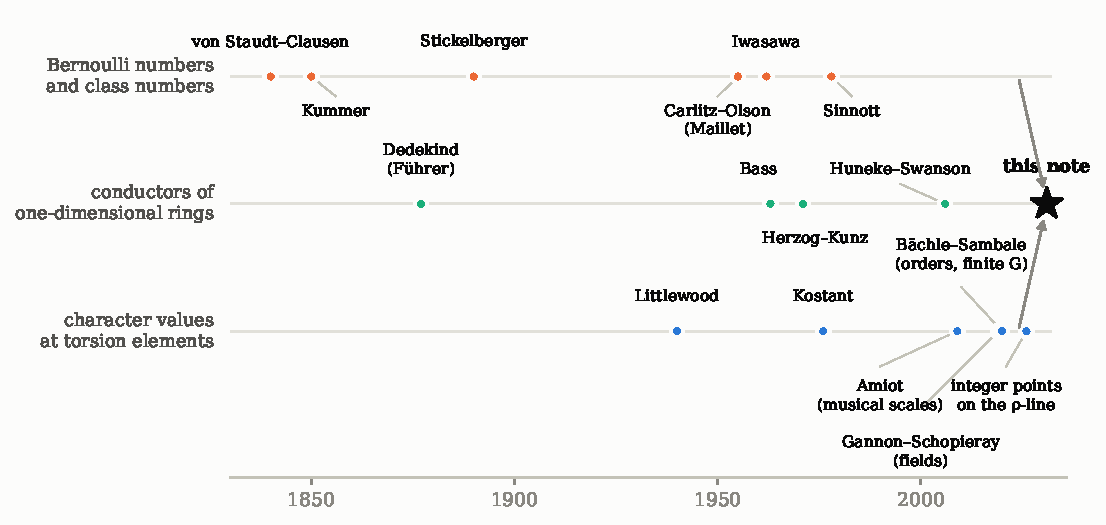
\includegraphics[width=\textwidth]{fig_historia.pdf}
\caption{Three lines of work, and the point where this note joins them. Dates are years of publication.}
\label{fig:historia}
\end{figure}

\noindent\textbf{Bernoulli numbers and class numbers.} The numbers $B_k$ enter number theory with von
Staudt and Clausen, who located their denominators, and with Kummer, who tied the divisibility of their
numerators by a prime $p$ to the class number of $\QQ(\zeta_p)$. Stickelberger's element annihilates the
class group; Iwasawa and Sinnott computed the index of the ideal it generates, which is the relative
class number $h^-$ up to a power of $2$ \cite{Sin78,Was97}. In between, Maillet asked for the
determinant of the matrix of least residues $R(rs^{-1})$, and Carlitz and Olson showed that it is a power
of $p$ times $h^-$ \cite{CO55}.

\noindent\textbf{Conductors of one-dimensional rings.} For a reduced one-dimensional ring $A$ with finite
normalisation $\cO$, the conductor $\cf=(A:\cO)$, Dedekind's \emph{Führer}, measures how far $A$ is from being
normal. Bass recorded, after Apéry, Gorenstein and Samuel,
that a Gorenstein ring satisfies $\ell(\cO/A)=\ell(A/\cf)$ \cite[Cor.~(6.5)]{Bas63}; Herzog and Kunz, and later
Huneke and Swanson, put the corresponding inequality and its equality case into the theory of the
canonical module \cite{HK71,HS06}.

\noindent\textbf{Character values at torsion elements.} Kostant singled out elements at which every
character of a simple group takes one of the values $0,\pm1$ \cite[Thm.~3.1]{Kostant76}; for $\Sp(2m)$ one of them,
the principal element of type $\rho$, is $g_{1/(2m+2)}$. The fields generated by character values are understood in the modular setting
\cite{GS19}, and for finite groups Bächle and Sambale studied the \emph{orders}
$\ZZ[\chi(g):\chi\in\mathrm{Irr}(G)]$ \cite{BS20}. For $\Sp(2m)$ along the line $g_{1/q}$, the points at
which every character is an integer were classified in \cite{Mar26}; a map of the older history of that
question is drawn there. Finally, from music theory: which intervals generate a given scale in $\ZZ/c$
was settled by Amiot \cite{Ami09}, and that is exactly the combinatorial lemma this note needs.

% ==============================================================================================
\section{When is the ring just \texorpdfstring{$\ZZ$}{Z}?}\label{sec:set}

\pregunta{Before asking what is missing, one should know when nothing is there to miss.}

\noindent Fix $q\ge3$, $1\le m<q/2$, $\xi=\xi_q$, $\eta_j=\xi^j+\xi^{-j}$, and $\cO=\ZZ[\xi+\xi^{-1}]$, the
ring of integers of $K=\QQ(\xi)^+$. The representation ring of $\Sp(2m)$ is $\ZZ[e_1,\dots,e_m]$, with $e_i$
the elementary symmetric functions of $x_1+x_1^{-1},\dots,x_m+x_m^{-1}$; hence
\begin{equation}\label{eq:A}
\marco{A=A_m(q)=\ZZ\bigl[e_1(\eta_1,\dots,\eta_m),\dots,e_m(\eta_1,\dots,\eta_m)\bigr]\subseteq\cO}
\end{equation}
Everything depends on how the segment $\{\pm1,\dots,\pm m\}$ sits modulo an integer $n$. Let
$N^{(n)}(c)=\#\{1\le j\le m: j\equiv\pm c\pmod n\}$ on classes $c\in(\ZZ/n)/\pm1$.

\begin{lemma}[segments]\label{lem:seg}
Let $n\ge3$ and let $a$ be a unit mod $n$ with $a\not\equiv\pm1$. Then $N^{(n)}$ is stable under $c\mapsto ac$
if and only if $n$ divides $h$, $h+1$ or $h+2$; in that case it is stable under every unit.
\end{lemma}

\begin{proof}
Write $m=kn+r$ with $0\le r<n$. Complete periods contribute a unit-invariant multiset, so stability is that
of the segment $\{\pm1,\dots,\pm s\}$ with $s=r$ if $r\le n/2$ and $s=n-1-r$ otherwise. The set $[-s,s]\subseteq\ZZ/n$
is a scale generated by $1$; if $a[-s,s]=[-s,s]$ it is also generated by $a$, and by \cite{Ami09},
Theorem~1, a coprime generator other than $\pm1$ forces the scale to have $1$, $n-1$ or $n$ elements. These
are $r\in\{0,n-1\}$, $r=(n-1)/2$ for odd $n$, and $r\in\{n/2-1,n/2\}$ for even $n$; that is, $n\mid h$, $n\mid
h+2$ or $n\mid h+1$. Those segments are stable under every unit. The same classification, with another proof,
is in \cite{Mar26}, Theorem~5.1.
\end{proof}

\noindent The musical reading is literal. In $\ZZ/12$ the diatonic scale $\{0,2,4,5,7,9,11\}$ is a run of seven
consecutive fifths, the scale Pythagorean tuning stacks: a segment for the generator $7$. It has seven notes, neither
$1$, $11$ nor $12$, so by Amiot's theorem no generator other than $\pm7$ lays it out as a segment. In the lemma the
roles are swapped: the segment $\{\pm1,\dots,\pm m\}$ is laid out by $1$, and the question is which other
generators it admits. The answer is governed by $h=2m$, the Coxeter number of type $C_m$, that is, the order of the
product of the simple reflections of its Weyl group.

\begin{table}[htbp]
\centering\small
\rowcolors{2}{filaclara}{white}
\begin{tabular}{llll}
\toprule
family & $m \bmod n$ & the segment $\{\pm1,\dots,\pm m\}$ mod $n$ & example ($m=6$) \\
\midrule
$n\mid h$ & $0$ or $n/2$ & whole periods ($+$ the class $n/2$) & $n=4,12$ \\
$n\mid h+1$ & $(n-1)/2$ & every nonzero class, once more & $n=13$ \\
$n\mid h+2$ & $n-1$ or $n/2-1$ & whole periods minus $\{0\}$ (and $\{n/2\}$) & $n=7,14$ \\
\bottomrule
\end{tabular}
\caption{The three stable families. $h=2m$ is the Coxeter number of type $C_m$.}
\label{tab:familias}
\end{table}

\begin{proposition}[$A=\ZZ$]\label{prop:AZ}
$A=\ZZ$ if and only if $q\in\{2m+1,2m+2\}$ or $(q,m)=(6,1)$. Otherwise $A$ is an order of rank $\varphi(q)/2$
in $K$.
\end{proposition}

\begin{proof}
The fraction field of $A$ is the fixed field of the stabiliser of $N^{(q)}$ in
$\mathrm{Gal}(K/\QQ)=(\ZZ/q)^\times/\pm1$. For $q\notin\{3,4,6\}$ Lemma~\ref{lem:seg} makes that stabiliser
trivial or everything, and with $2m<q$ it is everything exactly for $q\in\{2m+1,2m+2\}$. For
$q\in\{3,4,6\}$, $\cO=\ZZ$; with $2m<q$ this gives $m=1$ for $q=3,4$ and $m\in\{1,2\}$ for $q=6$.
\end{proof}

\noindent This is not new. For $m\ge2$ it is the part $2m<q$ of \cite{Mar26}, Theorem~5.1, whose
statement also contains a sporadic family $q=6$, $m\equiv1\pmod3$, outside the range $2m<q$ here; the
case $(6,1)$ is its $m=1$ shadow. In the language of rational elements it says that $g_{1/q}$ is conjugate
to all its prime-to-$q$ powers exactly at these points, and for $q=2m+2$ the element is one of Kostant's
\cite[Thm.~3.1]{Kostant76}. From now on $A\neq\ZZ$ and $\cf=(A:\cO)$.

\begin{lemma}[Galois stability]\label{lem:galois}
Assume $A\ne\ZZ$. The order $A$ and its conductor $\cf$ are stable under $\mathrm{Gal}(K/\QQ)$. Hence, for every prime $p$, all
primes of $\cO$ above $p$ occur in $\cf$ with the same exponent $e_p\ge0$: $\cf\,\cO_p=\rad_p^{\,e_p}$, where
$\rad_p$ is the radical of $\cO_p=\cO\otimes\ZZ_p$.
\end{lemma}

\begin{proof}
Let $C_u\in\ZZ[X]$ be Chebyshev's polynomial, rescaled so that $C_u(2\cos\theta)=2\cos u\theta$; equivalently
$C_u(t+t^{-1})=t^u+t^{-u}$, with $C_0=2$, $C_1=X$, $C_{u+1}=XC_u-C_{u-1}$. For $\sigma_u(\xi)=\xi^u$ one has $\sigma_u(\eta_j)=C_u(\eta_j)$, so
$\sigma_u(e_k(\eta_1,\dots,\eta_m))=e_k(C_u(\eta_1),\dots,C_u(\eta_m))$, a symmetric polynomial with integer
coefficients in $\eta_1,\dots,\eta_m$, hence an element of $A$. Thus $\sigma_u(A)\subseteq A$ for every $u$, and
equality follows by applying $\sigma_u^{-1}$. Then $\sigma_u(\cf)=(\sigma_u(A):\sigma_u(\cO))=\cf$, and the primes
above $p$ form one Galois orbit.
\end{proof}

\frontera{The integer points $q\mid h,h+1,h+2$ belong to type $C$. For another simply connected simple group, at which orders $q$ is $\exp(2\pi i\rho^\vee/q)$ conjugate to all its prime-to-$q$ powers, and can those $q$ be read off the regular numbers of its Weyl group?}

% ==============================================================================================
\section{Which primes divide the index?}\label{sec:sop}

\pregunta{The ring $A$ has finite index in $\cO$. Is there any pattern in the primes of that index?}

\noindent For a prime $p$ write $q=p^vq'$ with $p\nmid q'$, $E=\varphi(p^v)$, and let $f$ be the order of
$p$ in $(\ZZ/q')^\times/\pm1$, the residue degree of $p$ in $K$. Define, for $c\in\ZZ/q'$,
\begin{equation}\label{eq:S}
\marco{S(c)=\sum_{\substack{1\le j\le m\\ j\equiv c\ (q')}} j\;-\sum_{\substack{1\le j\le m\\ j\equiv -c\ (q')}} j}
\end{equation}
an odd function on $\ZZ/q'$: the first moment of the segment, class by class.

\begin{keybox}
\begin{theorem}[support of the conductor]\label{thm:sop}
Assume $A\ne\ZZ$.
\begin{enumerate}
\item[(a)] If $p\nmid q$, then $p\nmid[\cO:A]$.
\item[(b)] Let $p\mid q$ and $q'\ge3$. Then $p\mid[\cO:A]$ if and only if at least one of the following fails:
 \emph{(i)} the stabiliser of $N^{(q')}$ in $(\ZZ/q')^\times/\pm1$ is trivial;
 \emph{(ii)} $E=1$, or $S(c)\not\equiv0\pmod p$ for some $c$ with $2c\not\equiv0\pmod{q'}$.
\item[(c)] If $p\mid q$ and $q'\notin\{1,2,3,4,6\}$, then
 \[ p\mid[\cO:A]\iff q'\mid h,\ \ q'\mid h+1\ \ \text{or}\ \ q'\mid h+2 . \]
\end{enumerate}
\end{theorem}
\end{keybox}

\noindent Read through a prime $\mathfrak P$ of $\ZZ[\xi]$ above $p$, part~(c) says: reduction kills the
$p$-power part of $g$ and leaves its prime-to-$p$ part, of order $q'$; and for $q'\notin\{3,4,6\}$, $p$
divides the index exactly when that part lies on one of the three families $q'\mid h,h+1,h+2$ of integer points
(\cite{Mar26}, Theorem~5.1; Proposition~\ref{prop:AZ} is their part with $2m<q'$).
For the running example $A_3(35)$: at $p=7$ the part $q'=5$ divides none of $h,h+1,h+2=6,7,8$, so $7\nmid[\cO:A]$;
at $p=5$, $q'=7=h+1$, so $5\mid[\cO:A]$.
Figure~\ref{fig:paisaje} shows the index over the $(q,m)$-plane, split by prime and coloured by family.

\begin{proof}
Since $[\cO:A]$ is finite, $p\nmid[\cO:A]$ if and only if $A+p\cO=\cO$, i.e.\ the image of $A$ in $\cO/p\cO$ is
everything.

(a) For $p\nmid q$, $\cO/p\cO$ is étale and its $\overline{\FF}_p$-points are the reductions of
$\xi\mapsto\xi^u$, $u\in(\ZZ/q)^\times/\pm1$. At the point $u$ the $e_i$ are the elementary symmetric
functions of $u\cdot N^{(q)}$, and distinct multisets give distinct points because $c\mapsto
\omega^c+\omega^{-c}$ is injective on classes for a primitive root $\omega$ of order $q$ in characteristic $p$.
So $A$ generates $\cO/p\cO$ iff the stabiliser of $N^{(q)}$ is trivial, iff $A\ne\ZZ$ (Lemma~\ref{lem:seg},
Proposition~\ref{prop:AZ}). For the orders generated by all irreducible characters of a finite group $G$, the
analogous fact, that the primes of the index divide $|G|$, is \cite{BS20}, Proposition~6; it does not apply to $A$
directly, since $A$ is generated by characters of $\Sp(2m)$ only.

(b) In $\ZZ_p[\xi]$ write $\xi=\omega(1+\pi)$ with $\omega$ of order $q'$ and $1+\pi$ of order $p^v$; then
$\ZZ[\xi]/p=\FF_p[\omega][\pi]/(\pi^E)$. As $q'\ge3$, complex conjugation is not in the inertia group, so
$\cO/p\cO\cong\prod_{P\mid p}\FF_{p^f}[z]/(z^E)$ with $z=\eta_1-(\omega+\omega^{-1})\equiv(\omega-\omega^{-1})\pi$.
Let $\rad$ be the radical and $\bar R=\cO/\rad$ the residue ring. If $E=1$, then $\cO/p\cO=\bar R$ and only (i)
matters: the argument of (a) applies with $q'$ in place of $q$. Assume $E\ge2$, and let $B_2$ be the image of
$A$ in $\Lambda_2=\cO/(p,\rad^2)=\bar R[z]/(z^2)$. If $B_2=\Lambda_2$, then the image of $A$ in $\cO/p\cO$ contains
$\bar R$ (through $x\mapsto x^{p^N}$, which kills $z$) and a generator of $\rad/\rad^2$, hence everything;
the converse is clear. Modulo $\rad^2$, $\eta_j\equiv\gamma_j+jU_jz$ with $\gamma_j=\omega^j+\omega^{-j}$ and
$U_j=(\omega^j-\omega^{-j})/(\omega-\omega^{-1})$, so $\prod_j(T-\eta_j)\equiv F(T)-zG(T)$ with
$F=\prod_j(T-\gamma_j)$ and
\begin{equation}\label{eq:G}
\marco{G=F\sum_j\frac{jU_j}{T-\gamma_j}=F\sum_{c}\frac{S(c)\,U_c}{T-\gamma_c},}
\end{equation}
the second sum over classes with $N^{(q')}(c)\ge1$. The coefficients of $F$ generate $\bar R$ iff the
stabiliser of $N^{(q')}$ is trivial, as in (a). In that case $\bar R\subseteq B_2$, and the $z$-part of $B_2$
is the $\bar R$-submodule generated by the coefficients of $G$, which is all of $z\bar R$ iff $G$ is nonzero
in every residue field. The functions $U_cF/(T-\gamma_c)$ with $2c\not\equiv0$ and $N^{(q')}(c)\ge1$ are linearly
independent, so this happens iff $S(c)\not\equiv0\pmod p$ for some such $c$.

(c) By Lemma~\ref{lem:seg}, (i) fails iff $q'\mid h,h+1,h+2$. When (i) holds, $m=kq'+r$ with $r$ outside the
list of that lemma, and counting gives, for $1\le c\le q'-1$,
\[
S(c)=\begin{cases}(2k+1)c & c\le r<q'-c,\\ -(2k+1)(q'-c) & q'-c\le r<c,\\ (k+1)(2c-q') & q'-c\le r\ \text{and}\ c\le r,\\
k(2c-q') & r<c\ \text{and}\ r<q'-c.\end{cases}
\]
Write $n=q'$. Since $r\notin\{0,n-1\}$, the residue $c=1$ lies in the first case and $S(1)=2k+1$. If $r<n/2$
(so $r<(n-1)/2$ for odd $n$ and $r<n/2-1$ for even $n$), take $c=(n-1)/2$ for odd $n$, which gives $S(c)=-k$,
or $c=n/2-1$ for even $n$, which gives $S(c)=-2k$. If $r>n/2$,
take $c=(n+1)/2$ or $c=n/2+1$, which gives $S(c)=k+1$ or $2(k+1)$. In every case $p$ cannot divide both
$S(1)=2k+1$ and $S(c)$, since $\gcd(2k+1,k)=\gcd(2k+1,k+1)=1$. So (ii) holds whenever (i) does, for $p=2$ as
well.
\end{proof}

\begin{figure}[!htbp]
\centering
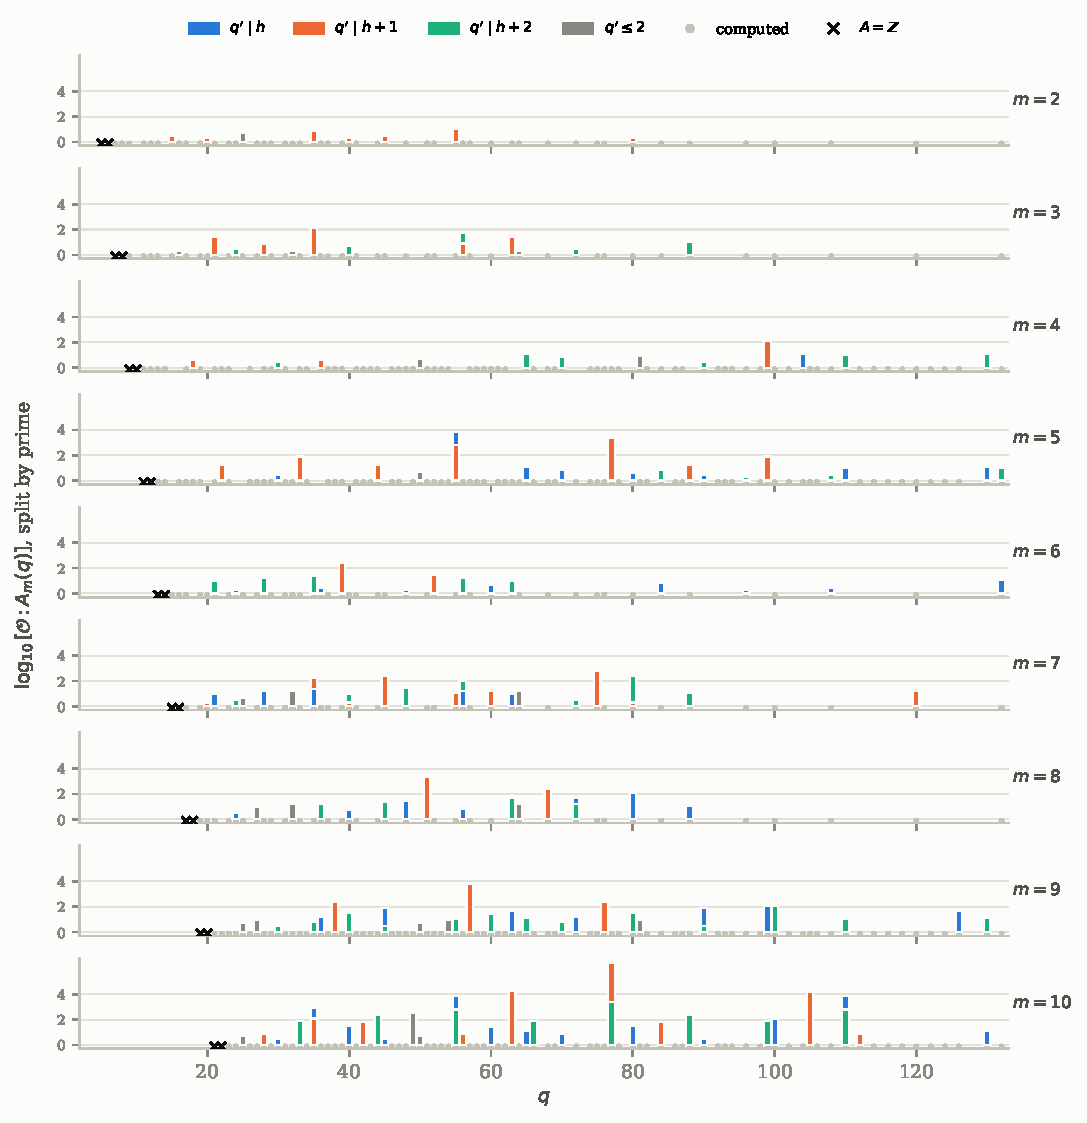
\includegraphics[width=\textwidth]{fig_paisaje2d.pdf}
\caption{The index $[\cO:A_m(q)]$ for $2\le m\le10$ and $q\le132$ ($558$ orders with a lattice computation, $156$
of them with index $>1$), one panel per $m$. Each bar is stacked by the primes $p$ of the index, each segment of
height $v_p\cdot\log_{10}p$ and coloured by the family of $q'=q/p^{v}$; grey segments are primes with $q'\le2$,
outside the theorems. Dots mark computed $q$ (no bar: index $1$); crosses mark $A=\ZZ$. Every coloured segment
lies over a pair with $q'\mid h,h+1,h+2$.}
\label{fig:paisaje}
\end{figure}

\frontera{Theorem~\ref{thm:sop}(b) has two clauses: an \'etale one, on the Galois stabiliser of the prime-to-$p$ part of $g$, and a tangent one, on the first moment. For a torsion element of any simply connected group, is $p\mid[\cO:\ZZ[\chi(g)]]$ still the failure of one of the two, with the differential of the fundamental characters in the role of $S$?}

% ==============================================================================================
\section{What does the defect look like at one prime?}\label{sec:loc}

\pregunta{Knowing that $p$ divides the index, one would like to see the conductor at $p$: how many maximal
ideals, which residue fields, how deep.}

\noindent Assume $p\mid q$, $q'\notin\{1,2,3,4,6\}$, $E\ge2$, and $q'\mid h,h+1,h+2$, so that $p\mid[\cO:A]$ and
$N^{(q')}$ is stable under every unit. Let $\rad$ be the radical of $\cO_p=\cO\otimes\ZZ_p$, $A_p=A\otimes\ZZ_p$,
$d=\varphi(q')/2=\dim_{\FF_p}\bar R$, and let $\gr_i(A)$ be the image of $A_p\cap\rad^i$ in
$\rad^i/\rad^{i+1}\cong\bar R$. Put $W_i=\dim_{\FF_p}\gr_i(A)$, so that $W_0=1$ and $W_i\le d$; by
Lemma~\ref{lem:galois}, $\cf\,\cO_p=\rad^{e}$ for a single exponent $e=e_p$.

\begin{keybox}
\begin{theorem}[local structure]\label{thm:loc}
Under these hypotheses:
\begin{enumerate}
\item[(a)] the image of $A$ in $\bar R$ is $\FF_p$; so $A$ has exactly one maximal ideal above $p$, it contains
 $\cf$, and its residue field is $\FF_p$;
\item[(b)] $W_1=\dim_{\FF_p}\FF_p[(\ZZ/q')^\times]\cdot S$, where $(u\cdot S)(c)=S(u^{-1}c)$;
\item[(c)] $e=1$ if and only if $W_1=d$;
\item[(d)] $v_p([\cO:A])=\sum_{i=0}^{e-1}(d-W_i)$ and $v_p([A:\cf])=\sum_{i=0}^{e-1}W_i$; in particular, if $e=2$,
 then $v_p([A:\cf])=1+W_1$ and $v_p([\cO:A])=2d-1-W_1$.
\end{enumerate}
\end{theorem}
\end{keybox}

\begin{proof}
(a) Stability makes $F\in\FF_p[T]$: the $e_i$ reduce to the same constants of $\FF_p$ in every residue field.
By Theorem~\ref{thm:sop}, $p\mid[\cO:A]$, so that ideal contains $\cf$.

(b) Every element of $A$ is $\Phi(e)$ with $\Phi\in\ZZ[X]$; modulo $\rad^2$,
$\Phi(e)\equiv\Phi(F)+z\sum_i(\partial_i\Phi)(F)G_i$ with $\Phi(F)\in\FF_p$, and $p\in\rad^2$. Hence $\gr_1(A)$ is
the $\FF_p$-span $V$ of the coefficients $G_i$. Since $\bar R$ is étale,
$\bar R\otimes_{\FF_p}\overline{\FF}_p\cong\overline{\FF}_p^{\,d}$, the coordinates being the $d$ embeddings
$\sigma_u\colon\omega+\omega^{-1}\mapsto\omega_0^u+\omega_0^{-u}$, $u\in(\ZZ/q')^\times/\pm1$, for a fixed
$\omega_0\in\overline{\FF}_p$ of order $q'$. Extension of scalars is injective on $\FF_p$-subspaces, so
$\dim_{\FF_p}V$ is the rank over $\overline{\FF}_p$ of the matrix whose row $u$ lists the coefficients of
$\sigma_u(G)$. Multiplying row $u$ by the unit $U_u$ does not change that rank. From
$\sigma_u(\gamma_c)=\gamma_{uc}$, $\sigma_u(U_c)=U_{uc}/U_u$ and the stability of $F$,
\begin{equation}\label{eq:rango}
\marco{U_u\,\sigma_u(G)=\sum_c S(u^{-1}c)\;U_c\,\frac{F(T)}{T-\gamma_c},}
\end{equation}
and the functions $U_cF/(T-\gamma_c)$, over the classes $c$ with $2c\not\equiv0\pmod{q'}$ (for the others $U_c=0$), are
linearly independent over $\overline{\FF}_p$ and do not depend on $u$.
So the rank equals that of $[S(u^{-1}c)]_{u,c}$, a matrix with entries in $\FF_p$, whose rank over
$\overline{\FF}_p$ equals its rank over $\FF_p$, which is $\dim_{\FF_p}\FF_p[(\ZZ/q')^\times]\cdot S$.

(c) If $\gr_1(A)=\gr_1(\cO)$, then $\gr_i(A)\supseteq\gr_1(A)^i=\gr_i(\cO)$ for all $i\ge1$, since $\gr(\cO_p)$ is a
polynomial ring over $\bar R$; so the closed sublattice $A_p\cap\rad$ has the graded of $\rad$ and equals it.
The converse is clear.

(d) Filter $\cO_p$ and $A_p$ by $\rad^i$. For $i\ge e$, $A_p\cap\rad^i=\rad^i$, so only the layers $i<e$
contribute: $\cO_p/A_p$ has a filtration with quotients of dimension $d-W_i$, and $A_p/\cf\cO_p=A_p/\rad^e$
one with quotients of dimension $W_i$.
\end{proof}

\noindent\textbf{The running example.} For $A_3(35)$ at $p=5$: $E=4$, $q'=7$, $d=3$, and since $m=3<7$ the first
moment is simply $S(c)=c$ for $c=1,2,3$ (and $S(-c)=-S(c)$). With rows $u=1,2,3$ and columns $c=1,2,3$, and
$u^{-1}\equiv1,4,5\pmod 7$,
\[
\bigl[S(u^{-1}c)\bigr]=\begin{pmatrix}1&2&3\\-3&1&-2\\-2&3&1\end{pmatrix},
\]
whose determinant is $0$ and whose rank is $2$ over $\QQ$ and modulo $5$. So $W_1=2<d=3$ and, by
Theorem~\ref{thm:loc}(c), the conductor at $5$ is not the radical. That the matrix is singular over $\ZZ$ itself is
explained in \S\ref{sec:clase}.

\noindent Products of layers make them usable in practice. Since $\gr(A)$ is a subring of
$\gr(\cO_p)$, the layers multiply: $\gr_i(A)\cdot\gr_j(A)\subseteq\gr_{i+j}(A)$. Write $\bar R=\prod_{a=1}^{g}k_a$ and
identify every layer with $\bar R$ through uniformisers $z_a$ of the factors; by Lemma~\ref{lem:galois} the group
$\mathrm{Gal}(K/\QQ)$ permutes the factors transitively and preserves $A_p\cap\rad^i$, acting on each layer by a
permutation of the factors, semilinear on each factor and twisted by units.

\begin{proposition}[growth of layers]\label{prop:cert}
Under the hypotheses of Theorem~\ref{thm:loc}, let $s\ge1$ with $W_s>0$. Then $W_{i+s}\ge W_i$ for all $i\ge0$. Hence:
\begin{enumerate}
\item[(a)] if $W_a=W_{a+1}=\dots=W_{a+s-1}=d$ for some $a$, then $\rad^a\subseteq A_p$ and $e\le a$; this applies with
 $s=E$, since $p\in A_p\cap\rad^E$ has nonzero image in $\gr_E(A)$;
\item[(b)] if $W_1>0$, then $e$ is the least $i$ with $W_i=d$.
\end{enumerate}
\end{proposition}

\begin{proof}
The image $V_s=\gr_s(A)\subseteq\bar R$ is nonzero and stable under the twisted action, so its projection to
every factor $k_a$ is nonzero. If $v_1,\dots,v_r$ is a basis of $V_s$, the element $v=\sum_k T^{k-1}v_k$ of
$\bar R\otimes_{\FF_p}\FF_p(T)=\prod_ak_a(T)$ has every component nonzero, so it is a unit, and multiplication by $v$
embeds $\gr_i(A)\otimes\FF_p(T)$ in $\gr_{i+s}(A)\otimes\FF_p(T)$; extension of scalars keeps dimensions, so
$W_i\le W_{i+s}$. (a) By induction every layer from $a$ on is full, and $A_p\cap\rad^a$, a closed sublattice with the
graded of $\rad^a$, equals $\rad^a$. Since the conductor commutes with $\otimes\ZZ_p$ and $\rad^a$ is an $\cO_p$-ideal,
$\rad^a\subseteq A_p$ gives $\rad^a\subseteq\cf\cO_p$, that is, $e\le a$. (b) Take $s=1$ in (a): a full layer $k$
gives $e\le k$; conversely $\rad^e\subseteq A_p$ makes $W_e=d$.
\end{proof}

\noindent Since $W_0=1<d$, the layers $0\le i<E$ contain at most $E-1$ full ones, so a computation limited to $i<E$
cannot use (a) with $s=E$; (b) needs only $W_1>0$ and one full layer. Several steps can be used at once.

\begin{corollary}[certifying by semigroups]\label{cor:semigrupo}
Under the hypotheses of Theorem~\ref{thm:loc}, let $\Sigma$ be the additive monoid (containing $0$) generated by the degrees $s\ge1$
with $W_s>0$. If $W_a=d$, then $W_{a+\sigma}=d$ for every $\sigma\in\Sigma$. In particular, if every degree $i\ge a$
is of the form $a'+\sigma$ with $W_{a'}=d$ and $\sigma\in\Sigma$, then $e\le a$.
\end{corollary}

\begin{proof}
Apply Proposition~\ref{prop:cert} once for each generator in a decomposition of $\sigma$; the last statement follows as
in Proposition~\ref{prop:cert}(a).
\end{proof}

\noindent A second product argument bounds the layers from above.

\begin{proposition}[complementary layers]\label{prop:mono}
Under the hypotheses of Theorem~\ref{thm:loc}, if $W_{i+j}<d$ then $W_i+W_j\le d$. In particular:
\begin{enumerate}
\item[(a)] $W_i+W_{e-1-i}\le d$ for $0\le i<e$, hence $2\sum_{i<e}W_i\le ed$;
\item[(b)] if $d/2<W_1<d$, then $e=2$.
\end{enumerate}
For $i+j=e-1$ the inequality is the diagonal case of \cite{CDK94}, Corollary~(3.7).
\end{proposition}

\begin{proof}
Extend scalars to $\overline{\FF}_p$, so that $\bar R\otimes\overline{\FF}_p=\overline{\FF}_p^{\,d}$ with coordinates
indexed by geometric points, permuted transitively by $\mathrm{Gal}(K/\QQ)$, and products of layers are computed
coordinatewise. If $V_{i+j}=\gr_{i+j}(A)\otimes\overline{\FF}_p$ is a proper subspace, its annihilator in the dual is
nonzero and stable under the twisted action; a generic linear combination of the translates of one nonzero
annihilating functional is a functional $\lambda(x)=\sum_a\lambda_ax_a$ in the annihilator with every
$\lambda_a\neq0$. The form $B_\lambda(x,y)=\lambda(xy)$ is nondegenerate, and $B_\lambda(V_i,V_j)\subseteq
\lambda(V_{i+j})=0$, so $W_i+W_j\le d$. (a) $W_{e-1}<d$: otherwise every layer from $e-1$ on would be full and
$\rad^{e-1}\subseteq A_p$, as in the proof of Proposition~\ref{prop:cert}(a). Summing over $i$ gives the second
inequality. (b) $2W_1>d$ forces $W_2=d$; by Proposition~\ref{prop:cert}(b), $e\le2$, and $e\ge2$ by
Theorem~\ref{thm:loc}(c).
\end{proof}

\begin{proposition}[one prime above $p$]\label{prop:unprimo}
Under the hypotheses of Theorem~\ref{thm:loc}, suppose that $p$ has a single prime above it in $K$, of prime
residue degree $f=d\ge3$, and that $2\le W_1<d$. Then $2\le e\le d-1$. In particular $e=2$ when $d=3$.
\end{proposition}

\begin{proof}
$\bar R=\FF_{p^d}$. Choose $a,b\in\gr_1(A)$ linearly independent over $\FF_p$ and put $t=b/a\notin\FF_p$; as $d$ is
prime, $t$ generates $\FF_{p^d}$, so $1,t,\dots,t^{d-1}$ is a basis. The products of $k$ elements of $\gr_1(A)$ lie
in $\gr_k(A)$ and include $a^k,a^{k-1}b,\dots,b^k=a^k(1,t,\dots,t^k)$, which span $\bar R$ once $k\ge d-1$. So every
layer $k\ge d-1$ is full, hence $\rad^{d-1}\subseteq A_p$ (as in the proof of Proposition~\ref{prop:cert}); and $e\ge2$ by Theorem~\ref{thm:loc}(c).
\end{proof}

\begin{proposition}[the Gorenstein criterion, in layers]\label{prop:gor}
Under the hypotheses of Theorem~\ref{thm:loc}, $A_p$ is Gorenstein if and only if $\ell(\cO_p/A_p)=\ell(A_p/\cf\cO_p)$,
that is, if and only if $2\sum_{i<e}W_i=ed$, that is, if and only if
\[
W_i+W_{e-1-i}=d\qquad\text{for every }0\le i<e .
\]
When $e=2$ this reads $W_1=d-1$.
\end{proposition}

\begin{proof}
That a Gorenstein ring is characterised by the length equality is classical: Bass proves one direction
\cite[Cor.~(6.5)]{Bas63} and records the converse there after Serre and Grothendieck; see also \cite{HK71} and
\cite{HS06}, Corollary~12.2.4. The symmetric form is the diagonal case of the criterion of Campillo, Delgado and
Kiyek \cite{CDK94}, (3.6)--(3.7), stated for analytically reduced one-dimensional local Cohen--Macaulay rings with
arbitrary residue extensions; we give a direct argument for the case at hand. By Theorem~\ref{thm:loc}(a), $R=A_p$ is local with residue field $\FF_p$; it is finite over $\ZZ_p$, hence complete,
reduced of dimension one, with finite normalisation $\cO_p$ and conductor $\cf\cO_p=\cf\otimes\ZZ_p$ (flat base
change). Every composition factor of a finite $R$-module is $\FF_p$, so its length is $\log_p$ of its cardinality; the
layers are killed by $p$, and there lengths are $\FF_p$-dimensions. So the first two forms of the condition agree
by Theorem~\ref{thm:loc}(d), and the third is the case of equality in Proposition~\ref{prop:mono}(a). If $R$ is Gorenstein the equality holds by
\cite[Cor.~(6.5)]{Bas63}, or \cite{HS06}, Theorem~12.2.2, which makes no assumption on the residue field. The converse
is \cite{HS06}, Corollary~12.2.4, for a one-dimensional analytically unramified local ring with infinite residue
field and a canonical module contained in the ring; we reach it through $S=R[T]_{\mathfrak mR[T]}$. The map $R\to S$
is flat and local with closed fibre $\FF_p(T)$. The ring $S$ is a localisation of a finitely generated algebra
over a complete local ring, hence excellent; being excellent and reduced, it is analytically unramified.
Its normalisation is the corresponding localisation of $\cO_p[T]$, which is normal and finite over $R[T]$. The
conductor is $\mathrm{Ann}_R(\cO_p/R)$, and annihilators of finitely generated modules commute with flat base
change, so the conductor of $S$ is $\cf S$. Lengths are preserved, since each composition factor $\FF_p$ becomes
$\FF_p(T)$. Finally $S$ is Cohen--Macaulay (reduced of dimension one), a quotient of a regular local ring, and generically
Gorenstein, so it has a canonical
module isomorphic to an ideal \cite[Thm.~3.3.6, Prop.~3.3.18(b)]{BH98}. Hence the equality for $R$ gives the equality for $S$, so $S$ is
Gorenstein by \cite{HS06}, Corollary~12.2.4, and so is $R$, because a flat local homomorphism of noetherian local
rings with Gorenstein target has Gorenstein source \cite[Tag~0BJL]{Stacks}.
\end{proof}

\begin{figure}[htbp]
\centering
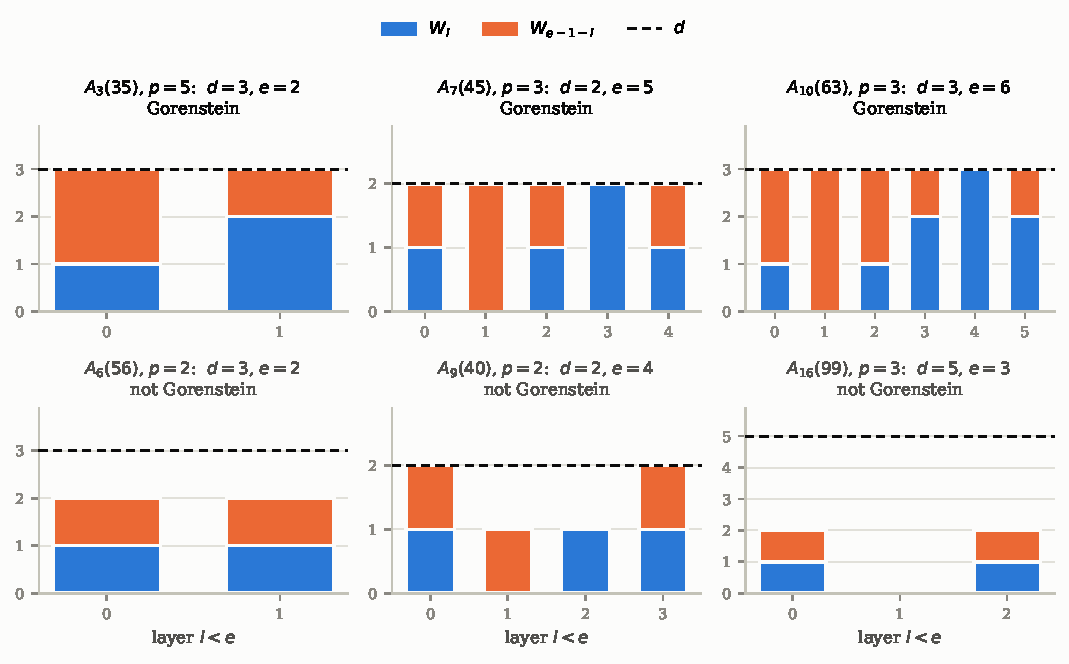
\includegraphics[width=\textwidth]{fig_simetria.pdf}
\caption{Proposition~\ref{prop:gor} on six lattice computations. Column $i<e$ stacks $W_i$ and its mirror $W_{e-1-i}$;
by Proposition~\ref{prop:mono} no column passes $d$, and the local ring is Gorenstein exactly when every column
reaches it. Top: $A_3(35)$, $A_7(45)$, $A_{10}(63)$; bottom: $A_6(56)$, $A_9(40)$, $A_{16}(99)$. In each panel the
symmetry agrees with $v_p([\cO:A])=v_p([A:\cf])$ computed on the lattice.}
\label{fig:simetria}
\end{figure}

\noindent The Gorenstein property is the case $\operatorname{type}(A_p)=1$ of a finer invariant. When the conductor is the
square of the radical, the type is read off the first layer and its multiplier ring.

\begin{proposition}[the type when $e=2$]\label{prop:tipo}
Under the hypotheses of Theorem~\ref{thm:loc}, suppose $e=2$. Let $V=\gr_1(A)\subseteq\bar R$ and
$\kappa=\dim_{\FF_p}\{a\in\bar R:\ aV\subseteq V\}$. Then the Cohen--Macaulay type of $A_p$ is
\[
\marco{\operatorname{type}(A_p)=d-W_1+\kappa-1,}
\]
$d-W_1\ge\kappa$, and $A_p$ is almost Gorenstein, $\ell(\cO_p/A_p)=\ell(A_p/\cf\cO_p)+\operatorname{type}(A_p)-1$,
if and only if $d-W_1=\kappa$.
\end{proposition}

\begin{proof}
Let $\mathfrak m=A_p\cap\rad$, the maximal ideal of $A_p$. Since $A_p\ne\cO_p$, $\mathfrak m$ is not invertible \cite[Lemma~2.14]{Mars24}, and by \cite{Mars24}, Proposition~3.5,
$\operatorname{type}(A_p)+1=\dim_{\FF_p}(\mathfrak m:\mathfrak m)/\mathfrak m$, and $(\mathfrak m:\mathfrak m)$, a ring
finite over $A_p$, lies in $\cO_p$. As $e=2$, $\rad^2\subseteq A_p$ and $\mathfrak m/\rad^2$ is the layer $V$. For
$x\in\cO_p$, $x\rad^2\subseteq\rad^2$, and $x\mathfrak m\subseteq\mathfrak m$ if and only if the residue $\bar x$
satisfies $\bar xV\subseteq V$. Hence $(\mathfrak m:\mathfrak m)=\{x\in\cO_p:\bar xV\subseteq V\}$ contains $\rad$, and
$\dim(\mathfrak m:\mathfrak m)/\mathfrak m=\kappa+(d-W_1)$. By Theorem~\ref{thm:loc}(d), $\ell(\cO_p/A_p)=2d-1-W_1$ and
$\ell(A_p/\cf\cO_p)=1+W_1$, so the almost Gorenstein equality reads $d-W_1=\kappa$. The inequality is
\cite{HS06}, Theorem~12.2.3, applied to $S=A_p[T]_{\mathfrak mA_p[T]}$ as in the proof of Proposition~\ref{prop:gor};
lengths and type do not change under that flat local extension with field fibre, because $\mathrm{Ext}$ commutes with
flat base change.
\end{proof}

\noindent The definition of almost Gorenstein rings is that of Barucci and Fröberg \cite{BF97}, in the length form used
by Marseglia \cite{Mars24}, \S7.2. On the $403$ pairs (order, prime) with $q\le250$ in which the computed layers certify $e=2$, the
type computed from the colon ideal modulo $\rad^2$ agrees with the formula, including $19$ with $\kappa>1$, $9$ of them
also by a colon on the lattice; so do the $63$ lattice pairs with $e=2$ (\emph{measured}, \S\ref{sec:metodo}).

% ==============================================================================================
\section{Why do class numbers appear?}\label{sec:clase}

\pregunta{Theorem~\ref{thm:loc} reduces the first layer, and with it the criterion for the conductor at $p$ to be
the radical, to the rank of a single matrix built from $S$.
Where have such matrices been seen before?}

\noindent Look at $S$ on the families of Table~\ref{tab:familias}. If $m=Nq'$ or $m=Nq'-1$, then
$S(c)=N(2c-q')$ for $1\le c\le q'-1$: up to the factor $2Nq'$, the sawtooth $B_1(c/q')$, whose coefficients are
those of Stickelberger's element. If $2m+1=Nq'$ with $q'$ odd, then $S(c)=N\hat c$, with $\hat c\in(-q'/2,q'/2)$
the signed residue: the same sawtooth shifted by half a period (Figure~\ref{fig:sierra}). For even $q'=2r$,
the two remaining stable families of Table~\ref{tab:familias}, $m=Br$ and $m=Br-1$ with $B$ odd, give the shifted
sawtooth of period $q'$ as well: $S(c)=B\,\hat s_{q'}(c)$, where $\hat s_{q'}(c)=\hat c$ is the signed residue modulo
$q'$ and $\hat s_{q'}(r)=0$.

\noindent Only these two functions occur, and one line says why. A sum is its count times its mean: writing $C(c)$
for the number of $j\in[-m,m]$ with $j\equiv c\pmod{q'}$ and $\mu(c)$ for the midpoint of that arithmetic
progression, $S(c)=C(c)\,\mu(c)$ whenever it is nonempty. What the family fixes is the midpoint. For
$m\equiv0,-1\pmod{q'}$ every class $c\neq0$ has $C(c)=2N$ and $\mu(c)=c-q'/2=s_{q'}(c)/2$; for $2m+1=Nq'$ every
class has $C(c)=N$ and $\mu(c)=\hat c$; on the half-period families $C(c)=B$ and $\mu(c)=\hat c$ away from the two
classes $0$ and $q'/2$ fixed by $c\mapsto-c$, where $S$ vanishes anyway. The sawtooth and its shift are the two
midpoints, and the multiplicity is the count.

\begin{figure}[htbp]
\centering
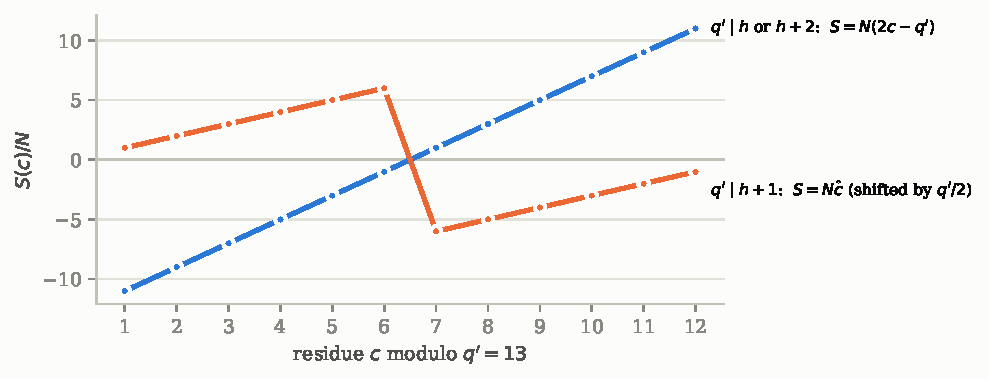
\includegraphics[width=0.78\textwidth]{fig_sierra.pdf}
\caption{The first-moment function $S$ for $q'=13$ on the two kinds of stable segment.}
\label{fig:sierra}
\end{figure}

\noindent For the first two families the matrix of Theorem~\ref{thm:loc}(b) is, up to the factor $N$, the
\emph{moment matrix}
\[
M_n=\bigl[s_n(u^{-1}c)\bigr],\qquad s_n(0)=0,\quad s_n(c)=2c-n\ (1\le c<n),
\]
with rows $u$ running over representatives of $(\ZZ/n)^\times/\pm1$ and columns over \emph{all} residues $1\le c<n$,
units or not. Its maximal minors are governed by Sinnott's index of the Stickelberger ideal.

\noindent The two kinds of segment lead to two different pieces of arithmetic. The answers, stated together:

\begin{keybox}
\begin{theorem}[class numbers]\label{thm:hminus}
Let $p$ be odd and $p\mid q$.
\begin{enumerate}
\item[(a)] If $q'\notin\{1,2,3,4,6\}$, $m\equiv0$ or $-1\pmod{q'}$ and $p\nmid N:=\lceil
 m/q'\rceil$, then $d-W_1$ is the number of elementary divisors of $M_{q'}$ divisible by $p$. The same holds on the
 half-period families: for $q'\ge8$ even, $r=q'/2$, $m\equiv r$ or $r-1\pmod{q'}$ and $p\nmid B:=\lceil
 m/r\rceil$. In both cases $\cf\,\cO_p=\rad$ if and only if $p\nmid h^-(\QQ(\zeta_{q'}))$.
\item[(b)] If $q'\ge5$ is prime and $2m+1=Nq'$ with $p\nmid N(q'-1)$, then
 \[W_1=\#\bigl\{\chi\ \text{odd mod}\ q' : (\overline\chi(2)-1)\,B_{1,\chi}\not\equiv0\pmod{\mathfrak p}\bigr\}\]
 for any prime $\mathfrak p$ above $p$ in $\QQ(\mu_{q'-1})$.
\end{enumerate}
\end{theorem}
\end{keybox}

\subsection{The sawtooth and Stickelberger's ideal}\label{sec:saw}

\begin{proposition}[Sinnott's index, on the moment matrix]\label{prop:sinnott}
Let $n\ge3$, $n\not\equiv2\pmod4$, $d=\varphi(n)/2$, and let $\Delta_n$ be the greatest common divisor of the
$d\times d$ minors of $M_n$. Then
\begin{equation}\label{eq:sinnott}
\marco{\Delta_n=2^{a}\,h^-(\QQ(\zeta_n))\,\frac{(2n)^d}{w_n},}
\end{equation}
where $w_n$ is the number of roots of unity in $\QQ(\zeta_n)$, $a=0$ if $n$ is a prime power and $a=2^{t-2}-1$ if $n$
has $t\ge2$ prime factors. In particular, for an odd prime $p\nmid n$, $v_p(\Delta_n)=v_p(h^-)$, and the rank of $M_n$
modulo $p$ is $d$ minus the number of elementary divisors of $M_n$ divisible by $p$.
\end{proposition}

\begin{proof}
This is Sinnott's index formula \cite{Sin78,Sin80} read through the generators of Bernard and Kučera \cite{BK24}.
Let $G=(\ZZ/n)^\times$ and, for $0<c<n$, $\omega_n(c)=\sum_{u\in G}\bigl(\langle-cu/n\rangle-\tfrac12\bigr)\sigma_u^{-1}$, with
$\langle x\rangle$ the fractional part. Replacing $u$ by $u^{-1}$ and using $\langle-x\rangle-\tfrac12=-(\langle
x\rangle-\tfrac12)$ for $x\notin\ZZ$,
\[
\sum_{u\in G}s_n(u^{-1}c)\,\sigma_u=-2n\,\omega_n(c),
\]
for units and non-units alike. Each $\omega_n(c)$ is odd, so the columns of $M_n$ are the coordinates of $-2n\,\omega_n(c)$
in the basis $\sigma_u-\sigma_{-u}$ of $R^-=\{\alpha\in\ZZ[G]:(1+\sigma_{-1})\alpha=0\}$, and $\Delta_n=[R^-:2n\Omega]$,
where $\Omega$ is the $\ZZ$-span of the $\omega_n(c)$. By \cite[Lemma~1.2 and (7)]{BK24}, Sinnott's group $S'$ is
generated by $\Omega$ and $\tfrac12N_G$; the Stickelberger ideal is $S=S'\cap\ZZ[G]$ \cite[\S1]{BK24}; since $\Omega$ is
odd and $N_G$ even, $S'\cap R^-\otimes\QQ=\Omega$ and $S^-=S\cap\Omega$; by \cite[Lemma~1.1]{BK24}
(\cite[Proposition~2.1]{Sin80}), $[S':S]=w_n$; and by \cite[(26)]{BK24}, from \cite{Sin78}, $[R^-:S^-]=2^ah^-$ with
$S^-=S\cap R^-$. An element $\alpha\in S$ with $(1+\sigma_{-1})\alpha=N_G$ \cite[Proposition~3.1]{BK24} puts
$\tfrac12N_G$ in $S+\Omega$, so $S'=S+\Omega$ and $[\Omega:S^-]=[S':S]=w_n$. As $\Omega$ has rank $d$ and
$2n\,\omega_n(c)=2n\,\theta_n(c)-n\,N_G\in S^-$,
$[S^-:2n\Omega]=(2n)^d/w_n$, and $\Delta_n=[R^-:S^-]\,[S^-:2n\Omega]$.
\end{proof}

\noindent The rectangular matrix itself is not new: Kuribayashi \cite{Kur08}, Proposition, proves that it has rank
$\varphi(n)/2$ over $\QQ$ for every $n>2$, in connection with a conjecture of Breuer \cite{Bre00}, Conjecture~C.12;
\eqref{eq:sinnott} refines that rank to the product of the elementary divisors, which is what the greatest common
divisor of the maximal minors is; how the $p$-part is distributed among them it does not say (\S\ref{sec:open}). The non-unit columns cannot be dropped: by
\cite[(6)]{BK24} they are the corestrictions of the
Stickelberger elements of the lower levels $n/\gcd(c,n)$, and without them the maximal minors may all vanish
(Remark~\ref{obs:comp}). \emph{Measured:} on the $66$ values $n<90$, $n\not\equiv2\pmod4$, the elementary divisors computed in Sage give
$v_p(\Delta_n)=v_p(h^-)$ for exact $h^-$ in all $1505$ pairs with $p$ odd, $p\le97$, $p\nmid n$, including the $40$
pairs with $p\mid\varphi(n)$, where the group algebra is not semisimple; the whole of~\eqref{eq:sinnott}, powers of $2$
and of $n$ included, holds on all $66$ (\S\ref{sec:metodo}).

\noindent Sinnott's normalisation excludes $n\equiv2\pmod4$, where $\QQ(\zeta_n)=\QQ(\zeta_{n/2})$. At odd primes
the moment matrix does not need the exclusion: doubling the period doubles its column lattice, although the power of $2$
in~\eqref{eq:sinnott} changes.

\begin{lemma}[half period, and doubling]\label{lem:dobla}
Let $n\ge4$ be even, let $\widehat M_n=\bigl[\hat s_n(u^{-1}c)\bigr]$, $0\le c<n$, and let $L_n$ and $L'_n$ inside
$\ZZ^{\varphi(n)/2}$ be the spans of the columns of $M_n$ and of $\widehat M_n$.
\begin{enumerate}
\item[(i)] For every $c$,
 \[
 \marco{\hat s_n(c)=\tfrac12\,s_n(c+n/2),\qquad\text{hence}\qquad L'_n=\tfrac12L_n.}
 \]
\item[(ii)] If $n=2r$ with $r\ge3$ odd, and the rows of $M_r$ and $M_{2r}$ are indexed by the same odd
 representatives $u$ of $(\ZZ/r)^\times/\pm1=(\ZZ/2r)^\times/\pm1$, then
 \[
 \marco{L_{2r}=2L_r,\qquad\text{hence}\qquad L'_{2r}=L_r.}
 \]
\end{enumerate}
So the elementary divisors of $\widehat M_n$ are half those of $M_n$, those of $M_{2r}$ are twice those of $M_r$,
$\Delta_{2r}=2^{d}\Delta_r$ with $d=\varphi(r)/2$, and for odd $p$ the matrices $M_n$ and $\widehat M_n$ --- and, for
$n=2r$, also $M_r$ --- have the same rank modulo $p$.
\end{lemma}

\begin{proof}
(i) For $0<c<n/2$ one has $c+n/2\in(n/2,n)$ and $s_n(c+n/2)=2c=2\hat s_n(c)$; for $n/2<c<n$ one has
$c+n/2\equiv c-n/2\in(0,n/2)$ and $s_n(c-n/2)=2c-2n=2\hat s_n(c)$; and both sides vanish at $c=0$ and at $c=n/2$, by
the conventions $s_n(0)=0$ and $\hat s_n(n/2)=0$. A unit $u$ modulo the even $n$ is odd, so $u^{-1}(c+n/2)=u^{-1}c+n/2$
and the identity holds entry by entry: the column $c$ of $\widehat M_n$ is half the column $c+n/2$ of $M_n$. Adjoining
to $M_n$ the zero column $c=0$, which does not change $L_n$, the map $c\mapsto c+n/2$ permutes the columns, so
$L'_n=\tfrac12L_n$; the halves are integral because $n$ is even, so every entry of $M_n$ is.

(ii) For $c$ modulo $r$ let $\nu(c)$ be the odd one of its two lifts modulo $2r$, and $c^*\in[0,r)$ the residue of
$2^{-1}c$, so that $c^*=(c+r)/2$ for odd $c\in[0,r)$ and $c^*=c/2$ for even $c$. Checking these two cases,
\[
s_{2r}(2c)=2s_r(c),\qquad s_{2r}(\nu(c))=2\bigl(s_r(c)-s_r(c^*)\bigr).
\]
As $u$ is odd, $u^{-1}\cdot2c=2(u^{-1}c)$ and $u^{-1}\nu(c)=\nu(u^{-1}c)$ modulo $2r$, and $(u^{-1}c)^*=u^{-1}c^*$
modulo $r$, so these identities hold column by column. The even columns of $M_{2r}$ are twice the columns of $M_r$,
all of them as $c$ runs over $\ZZ/r$, and its odd columns are twice differences of them, so $L_{2r}=2L_r$; with (i),
$L'_{2r}=\tfrac12L_{2r}=L_r$.
\end{proof}

\noindent \emph{Measured} for odd $r\le45$: the identities of (ii), the lattices, the elementary divisors and
$\Delta_{2r}$; and, end to end on the layers, in $304$ cases with $q'=2r$, $r\in\{5,7,11,13,23,29,31\}$ and
$p\in\{3,5,7\}$, in all four families (first layer only), including $p=3$ with $r=23,31$, where $p\mid h^-$. For (i):
the shift identity, $L'_n=\tfrac12L_n$, the elementary divisors and the equality of ranks at $p\le13$, on the $34$
even $n\le70$; and, end to end on the layers, in $158$ cases with $4\mid q'$, $q'\le88$, on the two half-period
families, among them the three pairs with $p\mid h^-$, namely $(q',p)=(52,3)$, $(64,17)$ and $(88,5)$, where
$W_1=d-1$ (\S\ref{sec:metodo}).

\noindent\textbf{One identity, two regimes.} Part~(i) and the Euler factor of \S\ref{sec:half} are the same identity.
For every $n$ and every $c$,
\[
\marco{2\,\hat s_n(c)=s_n(2c)-s_n(c),}
\]
the distribution relation of $B_1$ read on residues. What changes is whether $2$ is invertible modulo $n$. For $n$
odd, $c\mapsto2c$ permutes $\ZZ/n$ and the identity becomes $\bigl[\hat s_n(u^{-1}c)\bigr]=\tfrac12(P-I)M_n$ with $P$
the signed permutation of $u\mapsto u/2$; on characters it is the Euler factor $\overline\chi(2)-1$, which vanishes at
the odd characters trivial on $\langle2\rangle$, and that vanishing is the defect of Corollary~\ref{cor:dos}. For $n$
even, $c\mapsto2c$ is not injective, but $s_n(2c)-s_n(c)=s_n(c+n/2)$: the identity collapses to a translation by half
a period, which permutes the columns and cannot lose rank. So the factor at $2$ belongs to odd $q'$ alone, and the
same $\hat s$ serves both regimes. Nothing in the argument of Corollary~\ref{cor:dos} is special to $2$: for any
$\ell$ prime to $n$ the matrix of $\tfrac12\bigl(s_n(\ell c)-s_n(c)\bigr)$ has rank $\varphi(n)/2-\delta_\ell$ over
$\QQ$, and the same rank modulo every \emph{odd} prime $p\nmid n\,h^-$, with
$\delta_\ell=0$ if $-1\in\langle\ell\rangle$ and $\delta_\ell=\varphi(n)/(2\,\mathrm{ord}_n(\ell))$ otherwise
(\emph{measured} on the $52$ pairs $(n,\ell)$ with $n\le35$ odd and $\ell\le7$, over $\QQ$ and modulo the odd primes
$p\le13$ with $p\nmid n\,h^-$). The parity of $p$ is not cosmetic: for $n=5$ and $\ell=4$ the matrix has rows
$\pm(3,1,-1,-3)$, all entries odd, so its rank modulo $2$ is $1$, while $-1\in\langle4\rangle$ and $\delta_4=0$.
Only $\ell=2$ occurs here, because the only shift a symmetric segment can produce is half a period.

\begin{proof}[Proof of Theorem~\ref{thm:hminus}(a)]
Here $A\ne\ZZ$, and $E\ge2$ since $p$ is odd. In both families $S(c)=N\,s_{q'}(c)$ for $0\le c<q'$, so by Theorem~\ref{thm:loc}(b) $W_1$ is the rank modulo $p$ of $N M_{q'}$, which is that of $M_{q'}$
because $p\nmid N$; Proposition~\ref{prop:sinnott} (with $p\nmid q'$) and Theorem~\ref{thm:loc}(c) conclude. For
$q'=2r$ with $r$ odd, Proposition~\ref{prop:sinnott} does not apply at $q'$, but Lemma~\ref{lem:dobla}(ii) gives
$M_{q'}$ and $M_r$ the same number of elementary divisors divisible by $p$, and $\QQ(\zeta_{q'})=\QQ(\zeta_r)$, so it
applies at $r$ instead. On the half-period families, for any even $q'$, counting as in the proof of
Theorem~\ref{thm:sop}(c) gives $S=B\,\hat s_{q'}$ with $B=\lceil m/r\rceil$ odd: writing $m=kq'+r$ or $m=kq'+r-1$, the
$k$ complete periods contribute $k(2c-q')$ to $S(c)$ and the remaining segment contributes $kq'+c$ for $0<c<r$ and
$-(kq'+q'-c)$ for $r<c<q'$, so $S(c)=(2k+1)\hat c$ and $B=2k+1$. Hence $W_1$ is the rank modulo $p$ of
$\widehat M_{q'}$, which is that of $M_{q'}$ by Lemma~\ref{lem:dobla}(i). For $q'$
prime the block of $M_{q'}$ on $u,c<q'/2$ is $2$ times Maillet's reduced matrix up to transposition, and this is the
evaluation of Carlitz and Olson \cite{CO55}, (1.7) and (2.5).
\end{proof}

\begin{figure}[htbp]
\centering
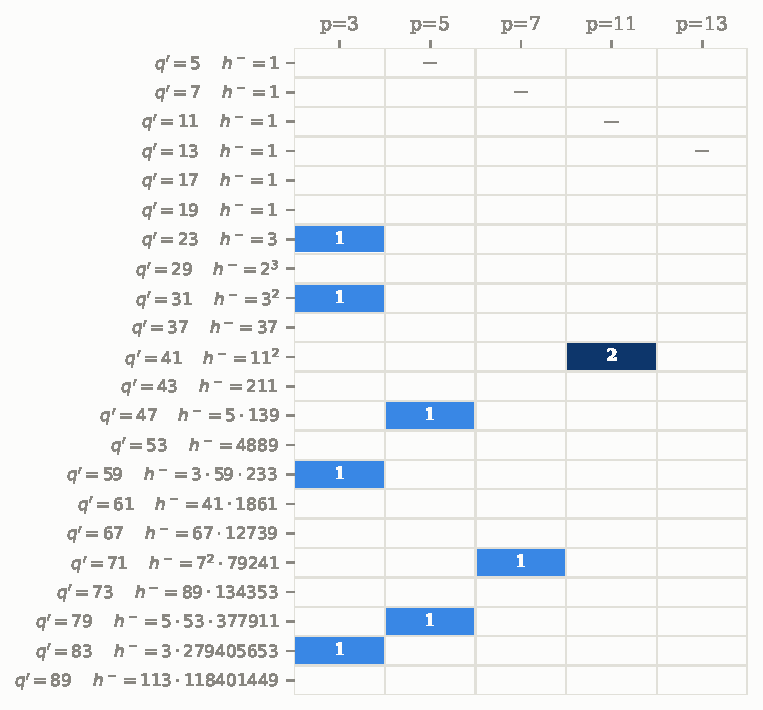
\includegraphics[width=0.72\textwidth]{fig_clase.pdf}
\caption{The defect $\varphi(q')/2-W_1$ for $S=2c-q'$, over primes $q'\le89$ and $p\le13$ (a dash where $p=q'$),
with $h^-(\QQ(\zeta_{q'}))$ beside each row. The nonzero cells are exactly the pairs with $p\mid h^-$.}
\label{fig:clase}
\end{figure}

\begin{remark}[squares and rectangles]\label{obs:comp}
For $q'$ prime, Proposition~\ref{prop:sinnott} is Carlitz and Olson's evaluation of Maillet's determinant. For
composite $q'$ the classical determinants are square. The matrix on units, evaluated by Tateyama and by Wang
\cite{Kuc01}, (2), vanishes as soon as some prime above $q'$ splits in $\QQ(\zeta_{q'})/\QQ(\zeta_{q'})^+$; Kučera's
determinants \cite{Kuc01}, Theorem~1, combine Stickelberger elements of all levels $n\mid q'$ with rational weights;
their value carries Euler factors $\prod(1-\overline\chi(\ell))$, which vanish for some choices of weights, and Kučera
chooses weights that give nonvanishing determinants for every conductor. Girstmair's index formula \cite{Gir89} uses
the conjugates of a single cotangent number inside the field, with explicit ramification factors. The rectangular
matrix $M_{q'}$, whose rank over $\QQ$ is Kuribayashi's \cite{Kur08}, spans $2q'\Omega$, of index $(2q')^d/w_{q'}$ in the minus part of the Stickelberger ideal, which is a
unit at every odd $p\nmid q'$; no choice of weights is needed. Figure~\ref{fig:stickel} shows it at work on the
non-prime values: an earlier measurement over $984$ pairs $(q',p)$ with $3\le q'<90$, $q'\not\equiv2\pmod4$ and odd
$p\le60$, $p\nmid q'$, is now a consequence of Proposition~\ref{prop:sinnott}.
\end{remark}

\begin{figure}[htbp]
\centering
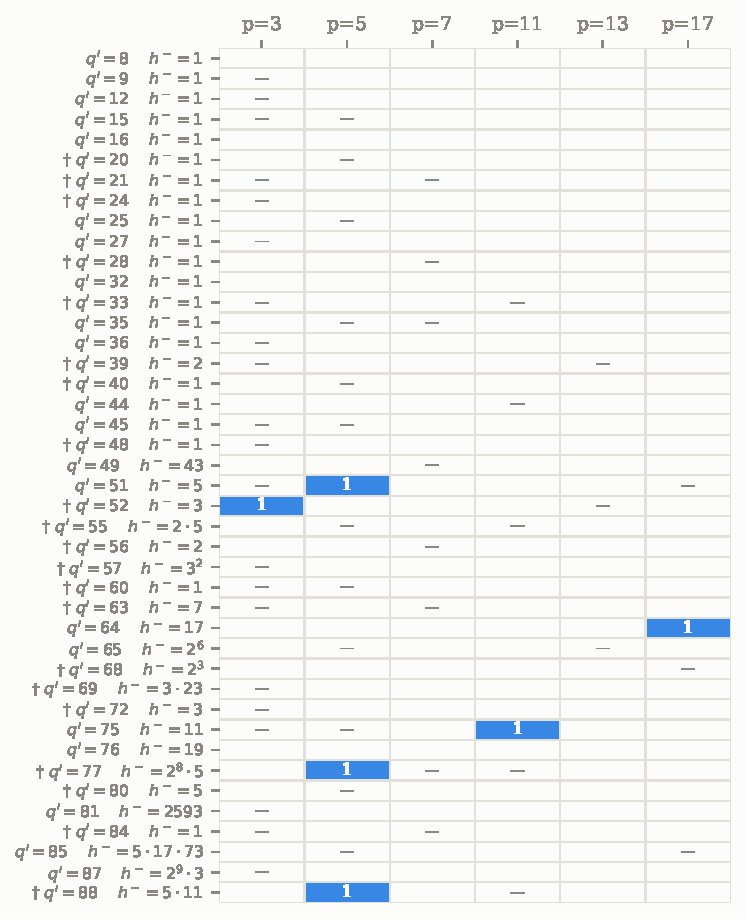
\includegraphics[width=0.74\textwidth]{fig_stickel.pdf}
\caption{Theorem~\ref{thm:hminus}(a) beyond prime $q'$: the rank defect of $M_{q'}$ modulo $p$, for the $42$ non-prime
$q'$ with $8\le q'<90$ and $q'\not\equiv2\pmod4$, and $p\le17$ (a dash where $p\mid q'$), with the exact
$h^-(\QQ(\zeta_{q'}))$ beside each row. The nonzero cells are exactly the pairs with $p\mid h^-$. A dagger marks
the $21$ values at which the square matrix on units alone is singular over $\QQ$.}
\label{fig:stickel}
\end{figure}

\noindent A simple divisor of the class number fixes the whole local picture.

\begin{corollary}[a simple divisor of $h^-$]\label{cor:simple}
In Theorem~\ref{thm:hminus}(a), suppose that $v_p(h^-(\QQ(\zeta_{q'})))=1$. Then $W_1=d-1$,
\[
\marco{\cf\,\cO_p=\rad^2,\qquad v_p([\cO:A])=v_p([A:\cf])=d,}
\]
and $A_p$ is Gorenstein.
\end{corollary}

\begin{proof}
By Proposition~\ref{prop:sinnott}, and Lemma~\ref{lem:dobla}(ii) when $q'\equiv2\pmod4$, exactly one elementary divisor
of $M_{q'}$ is divisible by $p$, so $W_1=d-1$ by Theorem~\ref{thm:hminus}(a). Since $p\mid h^-$ forces $d\ge3$ ($h^-=1$ when $\varphi(q')\le20$, \S\ref{sec:metodo}), $d/2<d-1<d$, and Proposition~\ref{prop:mono}(b) gives $e=2$;
Theorem~\ref{thm:loc}(d) gives the two lengths, and Proposition~\ref{prop:gor} with $W_1=d-1$ gives the Gorenstein
property.
\end{proof}

\noindent The hypothesis is sufficient, not necessary: a larger power of $p$ in $h^-$ can still leave a defect of
one (\emph{measured}: $(q',p)=(31,3)$ and $(71,7)$, with $v_p(h^-)=2$ and rank $d-1$). \textbf{A second example.} The running example $A_3(35)$ owes its defect to the factor at $2$, with $h^-=1$. The
order $A_{22}(69)$ owes it to the class number: $q=69$, $m=22\equiv-1\pmod{23}$, $p=3$, $N=1$, $d=11$ and
$h^-(\QQ(\zeta_{23}))=3$. Corollary~\ref{cor:simple} gives $W_1=10$, $\cf\,\cO_3=\rad^2=3\cO_3$,
$v_3([\cO:A])=v_3([A:\cf])=11$, and a Gorenstein ring $A_{22}(69)\otimes\ZZ_3$. A lattice computation, independent of
these arguments, returns $[\cO:A_{22}(69)]=3^{11}$, $\cf=3\cO$, layers $(W_0,W_1,W_2,W_3)=(1,10,11,11)$ and
Cohen--Macaulay type $1$ (\S\ref{sec:metodo}).
A class number can also leave a ring that is not almost Gorenstein. For $A_{40}(451)$ at $p=11$, with
$h^-(\QQ(\zeta_{41}))=11^2$, the layers give $W_1=18$ and $W_2=d=20$, so $e=2$; the multiplier ring of the first layer
is $\FF_{11}$, $\kappa=1$, and Proposition~\ref{prop:tipo} gives type $2$, while $\ell(\cO_{11}/A_{11})-\ell(A_{11}/\cf\cO_{11})=21-19=2\ne\operatorname{type}-1$
(\emph{computed} from the layers, not from a lattice).

\subsection{The shifted sawtooth and the factor at \texorpdfstring{$2$}{2}}\label{sec:half}

\begin{proof}[Proof of Theorem~\ref{thm:hminus}(b)]
The multiplication formula $B_1(2x)=B_1(x)+B_1(x+\tfrac12)$ gives
$\hat c/q'=B_1(\{c/q'+\tfrac12\})=B_1(\{2c/q'\})-B_1(\{c/q'\})$; summing against an odd character,
$\sum_c\chi(c)\hat c=q'(\overline\chi(2)-1)B_{1,\chi}$. This identity, with the same Euler factor, is in Kanemitsu and
Kuzumaki \cite{KK01}, proof of Theorem~1 ($t=2$, odd modulus), and in Kučera \cite{Kuc01}, Example~2, where it gives the
determinant of the square matrix of signed least residues; for the half sums $\sum_{a<q'/2}\chi(a)$ see
\cite{SUZ95}, (6). When $p\nmid q'-1$ the algebra $\FF_p[(\ZZ/q')^\times]$ is semisimple, and the dimension of
the cyclic module generated by the odd function $S$ is the number of odd characters at which its Fourier
transform is nonzero modulo $\mathfrak p$; the count does not depend on $\mathfrak p$, since Galois permutes the
characters.
\end{proof}

\noindent When the class number plays no role, the Euler factor makes everything explicit, with no condition on
$\varphi(q')$, and for composite $q'$ as well; what decides is the subgroup $\langle2\rangle$ of $(\ZZ/q')^\times$. When no
prime divisor of $q'$ splits in $\QQ(\zeta_{q'})/\QQ(\zeta_{q'})^+$ (for instance when $q'$ is a prime power), part~(a)
below also follows from the determinant of Kanemitsu--Kuzumaki and Kučera \cite{Kuc01}, (7) and Example~2, which is
then nonzero exactly when $-1\in\langle2\rangle$; part~(a) for the remaining composite $q'$, and the rank, lengths and
type in part~(b), we have not found.

\begin{corollary}[the factor at $2$]\label{cor:dos}
Let $p$ be odd, $p\mid q$, $q'\ge5$ odd, $2m+1=Nq'$ and $p\nmid N\,h^-(\QQ(\zeta_{q'}))$; let $t$ be the order of $2$
in $(\ZZ/q')^\times$ and $d=\varphi(q')/2$.
\begin{enumerate}
\item[(a)] If $-1\in\langle2\rangle$, then $W_1=d$ and $\cf\,\cO_p=\rad$.
\item[(b)] If $-1\notin\langle2\rangle$, put $\delta=d/t$. Then
\begin{equation}\label{eq:dos}
\marco{\begin{array}{c}W_1=d-\delta,\qquad \cf\,\cO_p=\rad^2,\\ v_p([\cO:A])=d+\delta-1,\qquad v_p([A:\cf])=d-\delta+1,\end{array}}
\end{equation}
and $A_p$ is almost Gorenstein of type $2\delta-1$; it is Gorenstein exactly when $\delta=1$.
\end{enumerate}
\end{corollary}

\begin{proof}
For every residue $c$ modulo $q'$ one has $\hat c=\tfrac12\bigl(s_{q'}(2c)-s_{q'}(c)\bigr)$. Hence, with rows $u$ over
representatives of $(\ZZ/q')^\times/\pm1$ and columns over all residues,
\[
\bigl[S(u^{-1}c)\bigr]=\tfrac N2\,(P-I)\,M_{q'},
\]
where $P$ is the signed permutation matrix of $u\mapsto u/2$. As $p\nmid h^-$, Proposition~\ref{prop:sinnott} makes
$M_{q'}$ of rank $d$ modulo $p$, so its columns span $\FF_p^d$, and the column space of $[S(u^{-1}c)]$ is the image of
$P-I$. Multiplication by $2$ splits $(\ZZ/q')^\times/\pm1$ into orbits. If $-1\in\langle2\rangle$ they have length
$t/2$ and $P$ has monodromy $-1$ along each ($2^{t/2}=-1$), so $P-I$ is invertible. If $-1\notin\langle2\rangle$, then
$2^k u\ne\pm u$ for $0<k<t$, so there are $\delta$ orbits of length $t$, with $t\ge3$ because $q'\nmid2^2-1$; $P$ has
monodromy $+1$, and the image of $P-I$ is the direct sum, over the orbits, of the hyperplanes
$\sum\epsilon_ux_u=0$ with all $\epsilon_u=\pm1$. By Theorem~\ref{thm:loc}(b) this gives $W_1$, and (a) follows from
Theorem~\ref{thm:loc}(c). In (b), $t\ge3$ gives $d/2<W_1<d$, so $e=2$ by Proposition~\ref{prop:mono}(b), and
Theorem~\ref{thm:loc}(d) gives the lengths. By~\eqref{eq:rango}, $V\otimes\overline{\FF}_p$ is this direct sum of
hyperplanes rescaled by the units $U_u^{-1}$ coordinatewise; a diagonal rescaling does not change the multiplier ring,
and the vectors $a$ with $aH\subseteq H$, for a hyperplane $H$ of $\overline{\FF}_p^{\,t}$ ($t\ge2$) with all coefficients nonzero, are the constants.
So $\kappa=\delta$, and Proposition~\ref{prop:tipo} gives type $2\delta-1$ and the almost Gorenstein equality.
\end{proof}

\noindent\textbf{The running example, concluded.} Take $q'=7$, $m=3$, $p=5$, so $q=35$ and $h^-(\QQ(\zeta_7))=1$. Here
$2m+1=7$, and the singular matrix of \S\ref{sec:loc} is explained by the odd character $\chi=\bigl(\frac{\cdot}{7}\bigr)$,
for which $\chi(2)=1$ kills the Euler factor. The
order of $2$ mod $7$ is $t=3$, so $-1\notin\langle2\rangle$, $\delta=1$, and Corollary~\ref{cor:dos}(b) gives $W_1=2$
and $e=2$. The order of $5$
in $(\ZZ/7)^\times/\pm1$ is $3=d$, so $5$ has a single prime above it, with residue field $\FF_{125}$. By
Theorem~\ref{thm:loc}(d),
\[
\cf\,\cO_5=\rad^2,\qquad v_5([A:\cf])=1+2=3,\qquad v_5([\cO:A])=6-1-2=3 ,
\]
so $[\cO:A_3(35)]=125$ and $[\cO:\cf]=5^6$, and by Proposition~\ref{prop:gor} the ring $A_3(35)\otimes\ZZ_5$ is Gorenstein. (The lattice computation
of \S\ref{sec:metodo} gives the same numbers.)

\noindent\textbf{A larger $\delta$.} For $A_{15}(155)$ at $p=5$: $q'=31$, $d=15$, $t=5$, $\delta=3$ and
$h^-(\QQ(\zeta_{31}))=9$. Here $5\mid q'-1$, outside Theorem~\ref{thm:hminus}(b), but inside Corollary~\ref{cor:dos}:
$W_1=12$, $\cf\,\cO_5=\rad^2$, $v_5([\cO:A])=17$, $v_5([A:\cf])=13$, and type $5$, so $A_{15}(155)\otimes\ZZ_5$ is almost
Gorenstein but not Gorenstein. A lattice computation returns $[\cO:A_{15}(155)]=5^{17}\cdot31$, $e_5=2$, layers
$(1,12,15)$ and type $5$ (\S\ref{sec:metodo}). The class number, by contrast, can break the almost Gorenstein equality
($A_{40}(451)$, \S\ref{sec:saw}).

\noindent\textbf{Composite $q'$.} For prime $q'$ the condition $-1\in\langle2\rangle$ says that $t$ is even; for composite
$q'$ it says more. For $q'=15$, $t=4$ but $2^2=4\ne-1$, so $\delta=1$: for $A_7(105)$ at $p=7$ the corollary gives
$W_1=3$, $e=2$, $v_7([\cO:A])=v_7([A:\cf])=4$ and a Gorenstein ring, and a lattice computation returns
$[\cO:A_7(105)]=7^4$, layers $(1,3,4)$ and type $1$. For $q'=63$, $t=6$ and $\delta=3$: the lattice of $A_{31}(315)$ at
$p=5$ has index $5^{20}$, layers $(1,15,18)$ and type $5$, as predicted. The hypothesis on $h^-$ is needed: with
$p\mid h^-$ the prediction fails in $3$ of $7$ controls, for instance $(q',p)=(77,5)$, where $W_1=28$ and not $29$.
\emph{Measured:} the layers $W_0,W_1,W_2$ agree with the corollary in all $1038$ cases computed, over odd $5\le q'<90$ other than $81$,
$p\le31$ and $N\le5$, with $13$ composite values of $q'$ at which $t$ is even and $-1\notin\langle2\rangle$; the type
$2\delta-1$, computed from the layers, agrees in the $26$ cases computed, with $\delta\le4$ (\S\ref{sec:metodo}).

\noindent Both corollaries end in the same two numbers, and so does the case $W_1=d$. Once the first layer is more
than half full, the index is settled.

\begin{corollary}[the index]\label{cor:indice}
Under the hypotheses of Theorem~\ref{thm:loc}, suppose $W_1>d/2$, or $W_1>0$ and $W_2=d$. Then $e\le2$ and
\[
\marco{v_p([\cO:A])=2d-1-W_1,}
\]
while $v_p([A:\cf])=1$ if $W_1=d$ and $1+W_1$ if $W_1<d$. The hypothesis holds in the families of
Theorem~\ref{thm:hminus}(a) as soon as $v_p(h^-(\QQ(\zeta_{q'})))<d/2$, and there
$v_p([\cO:A])=d-1+k$ with $k$ the number of elementary divisors of $M_{q'}$ divisible by $p$; it holds always in
Corollary~\ref{cor:dos}, where $v_p([\cO:A])=d-1+\delta$. Hence, if every prime of $q$ either fails the condition of
Theorem~\ref{thm:sop}(c) or satisfies these hypotheses,
\[
[\cO:A]=\prod_{p}p^{\,d_p-1+(d_p-W_1(p))},
\]
the product over the primes $p\mid q$ with $q'_p$ dividing $h$, $h+1$ or $h+2$, and $d_p=\varphi(q'_p)/2$.
\end{corollary}

\begin{proof}
If $W_1=d$ then $e=1$ by Theorem~\ref{thm:loc}(c) and Theorem~\ref{thm:loc}(d) gives $v_p([\cO:A])=d-W_0=d-1$,
which is $2d-1-W_1$. If $W_1<d$ then $e=2$: by Proposition~\ref{prop:mono}(b) when $d/2<W_1$, and by
Proposition~\ref{prop:cert}(b) when $W_1>0$ and $W_2=d$. Theorem~\ref{thm:loc}(d) then gives
$(d-1)+(d-W_1)$ and $1+W_1$. In Theorem~\ref{thm:hminus}(a), $d-W_1=k$ and each of those $k$ elementary divisors
contributes at least one factor $p$ to $\Delta_{q'}$, so $k\le v_p(\Delta_{q'})=v_p(h^-)$ by
Proposition~\ref{prop:sinnott}, and $v_p(h^-)<d/2$ gives $W_1>d/2$. In Corollary~\ref{cor:dos},
$d-W_1=\delta=d/t$ with $t\ge3$, so $W_1\ge2d/3$. The last formula is Theorem~\ref{thm:sop}(a) and~(c), which leave
no other primes.
\end{proof}

\noindent \emph{Measured} against the lattice: on the $104$ pairs (order, prime) of the index sweep with $p$ odd,
$q'\notin\{1,2,3,4,6\}$ and $W_1>d/2$, the formula gives the exponent of the lattice index in every case, and the
explicit form does so in the $103$ of them with $p\nmid N$ (or $p\nmid B$) and, in the centred family, $p\nmid h^-$;
the three pairs of the sweep outside the hypothesis all have $W_1=0$ and $p\mid N$, where
Propositions~\ref{prop:escalera} and~\ref{prop:descenso} take over. Figure~\ref{fig:zonas} places the measured
profiles on the first-layer axis: of the $168$ with $q'\notin\{1,2,3,4,6\}$, $126$ have $W_1=d$ and $18$ have
$d/2<W_1<d$, so the first clause decides them; the $17$ with $0<W_1\le d/2$ all have $p=2$, and the second clause
decides the $10$ of them whose $W_2$ is within the computed range, always $d$ (in the other $7$, $E=2$, and the
lattice lengths are those of $e=2$); the remaining $7$ have $W_1=0$ (\S\ref{sec:metodo}).

\begin{figure}[htbp]
\centering
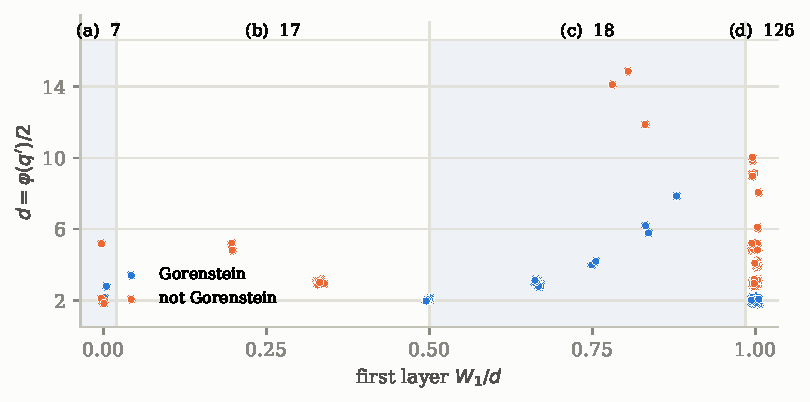
\includegraphics[width=0.86\textwidth]{fig_zonas.pdf}
\caption{Where the first layer falls, on the $168$ measured profiles with $q'\notin\{1,2,3,4,6\}$, and what decides
the exponent in each band: (a) $W_1=0$, the zone of the ladder and the descent (Propositions~\ref{prop:escalera}
and~\ref{prop:descenso}); (b) $0<W_1\le d/2$, where Corollary~\ref{cor:indice} needs its second clause $W_2=d$;
(c) $d/2<W_1<d$, where Proposition~\ref{prop:mono}(b) gives $e=2$; (d) $W_1=d$, where $e=1$. Colour marks whether
the local ring is Gorenstein. The vertical axis is $d=\varphi(q')/2$, with a small jitter so that repeated pairs
separate.}
\label{fig:zonas}
\end{figure}

\frontera{Theorem~\ref{thm:hminus} lives on one line of one group. On the principal line of an exceptional group, is there an order at which a prime dividing a relative class number enters the conductor, and which Euler factor then plays the role of $\overline\chi(2)-1$?}

% ==============================================================================================
\section{What lies beyond the first layer?}\label{sec:capas}

\pregunta{The first layer is now tied to class numbers, and it fixes the exponent when it is full or more than
half full. What do the deeper layers look like?}

\noindent\textbf{Observed and certified.} A finite window of layers does not decide the exponent in general:
$A_7(45)$ at $p=3$ has $(W_1,\dots,W_5)=(0,1,2,1,2)$ with $d=2$, so a full layer can be followed by a deficient
one; its lattice computation gives $\cf\,\cO_3=\rad^5$. Call \emph{observed exponent} the first level from which
all computed layers are full. In $1183$ pairs (order, prime) whose layers were computed, most of them without a lattice computation
($p\le7$, $q'\le24$, $q\le260$, layers $i\le6$), all $215$ with $1\le W_1<d$ and at least four computed layers
have observed exponent $2$ ($34$ more have too few layers to say). In all $215$, Proposition~\ref{prop:cert}(b),
applied to the computed $W_1>0$ and $W_2=d$, certifies $e=2$, also in the $10$ with several primes above $p$. What
makes that second layer full is the ring structure alone: \emph{measured} on $238$ pairs with $p\nmid N$,
$\gr_2(A)=\gr_1(A)\cdot\gr_1(A)$, so no new generator appears in degree $2$, and that product is the whole of $\bar R$
in all of them. It is not full \emph{because} the layer is nonzero, though: a stable line is its own square up to a
scalar, and the ladder produces exactly that, $\gr_{P-p^j}(A)$ being a line by Proposition~\ref{prop:escalera}, which
is why the exponent is large there. So the hypothesis of Corollary~\ref{cor:indice} cannot be weakened to
$\gr_1(A)\neq0$; on the families of Theorem~\ref{thm:hminus}(a) it says that fewer than $d/2$ elementary divisors of
$M_{q'}$ are divisible by $p$, and since that number is at most $v_p(h^-)$, removing it would take a bound on the
$p$-rank of the minus class group. \emph{Measured}: among $359$ stable subspaces of $\bar R$ generated by random
vectors, over $q'\le25$ and $p\le11$, every one with $\dim V>d/2$ squares to $\bar R$, while $7$ of the $9$ with
$\dim V\le d/2$ do not (\S\ref{sec:metodo}). For $p\in\{2,3,5\}$, $q'\in\{5,7,9,11,13\}$ and layers $i\le11$, the computed
profile depends only on $p$, $q'$, the family and $v_p(N)$, and the observed exponent is often, but not always,
$e_0\,p^{v_p(N)}$, where $e_0$ is the observed exponent with $v_p(N)=0$.

\begin{figure}[htbp]
\centering
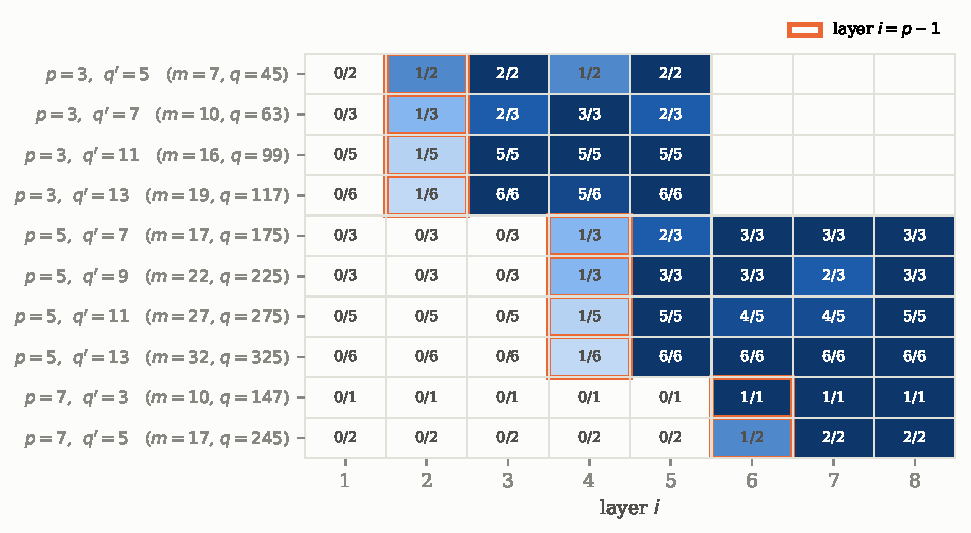
\includegraphics[width=0.86\textwidth]{fig_perfil.pdf}
\caption{Layers $W_i$, written as $W_i/d$, for ten orders with $p$ odd and $v_p(N)=1$. Every layer of positive degree below $p-1$
vanishes and layer $p-1$ (framed) has dimension $1$, as Proposition~\ref{prop:escalera} proves when $q'\ge5$. Only layers $i<E=\varphi(p^v)$ were computed, which is why the
rows with $p=3$ ($E=6$) stop at $i=5$. The rows show layers, not certified exponents
(Proposition~\ref{prop:cert}).}
\label{fig:perfil}
\end{figure}

\noindent\textbf{What the figure already certifies.} Corollary~\ref{cor:semigrupo} turns some rows of
Figure~\ref{fig:perfil} into exponents without computing further layers. For $A_{10}(63)$ at $p=3$ the layers are
$(1,0,1,2,3,2)$ with $d=3$: $W_2,W_3>0$ and $W_4=d$, and $\langle2,3\rangle$ contains every integer $\ge2$, so every
layer from $4$ on except possibly $5$ is full; $W_5=2$, so $e=6$, $\cf\,\cO_3=\rad^6=3\cO_3$, and by
Proposition~\ref{prop:gor} $A_{10}(63)\otimes\ZZ_3$ is Gorenstein. In the same way the rows give $e=5$ for
$A_7(45)$, $e=3$ for $A_{16}(99)$ and $e=5$ for $A_{19}(117)$ at $p=3$, and $e=8$ for $A_{22}(225)$ and $A_{27}(275)$ and
$e=5$ for $A_{32}(325)$ at $p=5$; the rows of $A_{17}(175)$ and $A_{17}(245)$ only bound $e$, and $A_{10}(147)$ has $q'=3$, outside
Theorem~\ref{thm:loc}. Lattice computations
confirm the five values that are within reach ($A_7(45)$, $A_{10}(63)$, $A_{16}(99)$, $A_{19}(117)$, $A_{22}(225)$).

\noindent The first zone of these profiles is not an accident of the examples: before degree $p^{v_p(N)}$ it is
universal.

\begin{proposition}[a universal ladder]\label{prop:escalera}
Let $A\ne\ZZ$, let $p$ be odd, $q'\ge5$ odd, $2m+1=Nq'$ with $N=p^aM$, $a\ge1$, $p\nmid M$, and $q=p^vq'$; put
$P=p^a$. Then $v>a$, because $A\ne\ZZ$ forces $q>2m+1$ by Proposition~\ref{prop:AZ}, that is $p^aM<p^v$; and
$W_0=1$ and, for $1\le i<P$,
\[
\marco{W_i=\begin{cases}1,& i\in\{P-p^j:\ 0\le j<a\},\\ 0,&\text{otherwise,}\end{cases}}
\]
In particular the first nonzero layer of positive degree is $W_{\varphi(P)}=1$, and the image of $A_p$ in $\cO_p/\rad^P$ is the ring
\[
\FF_p[\epsilon_0,\dots,\epsilon_{a-1}]/(\epsilon_i\epsilon_j:\ 0\le i,j<a),
\]
with $\epsilon_j$ in degree $P-p^j$.
\end{proposition}

\begin{proof}
Put $Q_m(T)=\prod_{j=-m}^m(T-\xi^j)=(T-1)\,T^m\prod_{j=1}^m\bigl(T+T^{-1}-\eta_j\bigr)$; the passage between the
coefficients of $Q_m$ and the $e_k$ is triangular over $\ZZ$, so they generate the same ring $A$. Work in $\ZZ[\xi]$,
unramified over $\cO$ above $p$, with $\xi=\omega\rho$, $\omega$ of order $q'$, $\rho$ of order $p^v$ and uniformiser
$\pi=\rho-1$. Since $E=\varphi(p^v)\ge P$, layers below $P$ only see the image of $A$ in $\ZZ[\xi]/(p,\pi^P)
=\FF_p[\omega]\otimes\FF_p[\rho]/(\rho^P-1)$, where $\xi$ has order $q'P$. The $2m+1=Mq'P$ consecutive exponents cover
every residue modulo $q'P$ exactly $M$ times, so the coefficients of $Q_m$ are invariant under $(\ZZ/q'P)^\times$,
which acts on the two factors separately. The invariants of $\FF_p[\omega]$ are $\FF_p$; those of $\FF_p[\rho]/(\rho^P-1)$
are spanned by the sums over the subgroups $p^j\ZZ/P$, $\sum_{p^j\mid i}\rho^i=(\rho^P-1)/(\rho^{p^j}-1)=\pi^{P-p^j}$,
$0\le j\le a$, the last of which is $1$. The products of the $a$ nonconstant ones, $0\le i,j<a$, vanish modulo
$\pi^P$ because $p^i+p^j\le2P/p<P$, which gives the upper bound and the ring structure. For the lower
bound take one block, $L=q'P$: by the $q$-binomial theorem the coefficients of $\prod_{j=0}^{L-1}(T-\xi^j)$ are, up to
units, $\genfrac{[}{]}{0pt}{}{L}{k}_\xi=\prod_{i=1}^k(1-\xi^{L-k+i})/(1-\xi^i)$. Here $1-\xi^i$ is a unit unless $q'\mid i$, and then
$v_\pi(1-\xi^i)=p^{v_p(i)}$ because $v_p(i)\le a<v$. Pairing $i$ with $L-i$, which have the same $v_\pi(1-\xi^i)$ for $0<i<L$
(if $q'\mid i$ then $v_p(i)<a$), leaves $v_\pi\genfrac{[}{]}{0pt}{}{L}{k}_\xi=P-p^{v_p(k)}$ if $q'\mid k$ and $P$ otherwise. For $k=q'p^j$ this is
$P-p^j$. Modulo $\pi^P$ the full product is the $M$-th power of a shifted block, $(T^L-1+X)^M\equiv(T^L-1)^M+
M(T^L-1)^{M-1}X$, since the coefficients of $X$ have valuation at least $P-p^{a-1}\ge P/2$; its coefficient of
$T^{q'p^j}$ is $\pm M$ times that of $X$, of valuation exactly $P-p^j$, and $M$ is a unit.
\end{proof}

\noindent For $a=1$ this is the observation $W_{p-1}=1$ of Figure~\ref{fig:perfil}; for $a=2$ and $p=3$ the nonzero
layers of positive degree below $9$ are $W_6$ and $W_8$. The first nonzero term is itself a classical object: \emph{measured} in $16$
cases, any block of $q'P$ consecutive exponents, here the centred one, satisfies
\[
\prod_{|j|\le(q'P-1)/2}(T-\xi^j)\equiv T^{q'P}-1+\pi^{\varphi(P)}\,\mathrm{li}_1\bigl(T^{q'p^{a-1}}\bigr)
\pmod{\pi^{\varphi(P)+1}},\qquad \mathrm{li}_1(X)=\sum_{r=1}^{p-1}\frac{X^r}{r},
\]
the finite logarithm of Kontsevich, in Besser's notation \cite{Bes02}.

\noindent At degree $p^{v_p(N)}$ itself the arithmetic of the first moment comes back, as the first layer of a smaller
order of the same family.

\begin{proposition}[descent to the reduced segment]\label{prop:descenso}
Under the hypotheses of Proposition~\ref{prop:escalera}, put $m_0=(Mq'-1)/2$, $q_0=q/P$ and $A_0=A_{m_0}(q_0)$. Then
\[
\marco{W_P\bigl(A_m(q)\bigr)=W_1(A_0)=\dim_{\FF_p}\FF_p[(\ZZ/q')^\times]\cdot S_0,\qquad S_0(c)=M\hat c,}
\]
both layers taken at $p$. Moreover, with $w=W_1(A_0)$, the ring $A_p/(A_p\cap\rad^{P+1})$ is $\FF_p$ plus an ideal of
square zero with a basis $\epsilon_0,\dots,\epsilon_{a-1},\delta_1,\dots,\delta_w$, of filtration degrees $P-p^j$ and $P$.
\end{proposition}

\begin{proof}
Keep the notation of the proof of Proposition~\ref{prop:escalera}, with $n=q'$ and
$k=\FF_p[\omega]=\FF_p[X]/(\overline\Phi_n(X))$, $\omega=X$: a product of $g$ copies of $\FF_{p^f}$, one for each prime
above $p$, not a single field. Write $\iota$ for the involution $\omega\mapsto\omega^{-1}$ of $k$ and $k^\pm$ for its
$\pm1$-eigenspaces, so that $k=k^+\oplus k^-$ because $p\neq2$. As $v\ge a+1$,
$E\ge2P\ge P+1$, so $p\in\pi^{P+1}$ and $\Lambda=\ZZ_p[\xi]/(\pi^{P+1})=k[\pi]/(\pi^{P+1})$; the image $B$ of $A_p$ in
$\Lambda$ is the $\FF_p$-algebra generated by the coefficients of $Q_m$, and for $i\le P$, $\gr_i(A)$ is the image of
$B\cap\pi^i\Lambda$ in $\pi^i\Lambda/\pi^{i+1}\Lambda=k$.

\emph{Blocks.} Put $\ell=Mn=2m_0+1$ and $b=(P-1)/2$. Every integer in $[-m,m]$ is $c+\ell j$ for exactly one pair
$|c|\le m_0$, $|j|\le b$. With $\tau=\xi^\ell=\rho^\ell$, a primitive $p^v$-th root of unity, write
$\prod_{|j|\le b}(Z-\tau^j)=Z^P-1+\sum_{k=1}^{P-1}b_kZ^{P-k}$. Then
\begin{equation}\label{eq:bloques}
Q_m(T;\xi)=\prod_{|c|\le m_0}\bigl(T^P-\xi^{cP}+E_c(T)\bigr),\qquad E_c(T)=\sum_{k=1}^{P-1}b_k\,\xi^{ck}\,T^{P-k},
\end{equation}
and the valuation argument of Proposition~\ref{prop:escalera}, applied to $\genfrac{[}{]}{0pt}{}{P}{k}_\tau$, gives
$v_\pi(b_k)=P-p^{v_p(k)}\ge s:=P-P/p$, with $2s>P$. So, modulo $\pi^{P+1}$, only the terms with at most one factor $E_c$
survive. With $\zeta=\omega^P$, $\xi_0=\xi^P$ and $F_c(Y)=\prod_{c'\ne c}(Y-\xi_0^{c'})$,
modulo $\pi^{P+1}$
\[
[T^{Pj}]\,Q_m(T;\xi)\equiv[Y^j]\,Q_{m_0}(Y;\xi_0),\qquad
[T^{Pj+P-k}]\,Q_m(T;\xi)\equiv b_k\sum_{|c|\le m_0}\xi^{ck}\,[Y^j]\,F_c(Y).
\]

\emph{Partial fractions.} Let $F(Y)=\prod_{|c|\le m_0}(Y-\zeta^c)=(Y^n-1)^M$ and $G_h=\sum_{c\in\ZZ/n}S_0(c)\zeta^{ch}$.
Grouping $c$ by residues, $\sum_{|c|\le m_0}\zeta^{ch}F(Y)/(Y-\zeta^c)=Mn\,(Y^n-1)^{M-1}Y^{i_h}$ with $i_h\equiv h-1$,
an integer polynomial, and $D_h(Y)=\sum_{|c|\le m_0}c\,\zeta^{ch}F(Y)/(Y-\zeta^c)=(Y^n-1)^{M-1}\sum_{i<n}G_{h-1-i}Y^i$.
Let $V\subseteq k$ be the span of the residues of the $G_h$; the coefficients of every $D_h$ lie in $V$, and those of
$D_1$ in degrees $n(M-1)+i$ are the $G_{-i}$, so they span $V$. As $S_0$ is odd, $G_h$ is anti-invariant under
$\omega\mapsto\omega^{-1}$; so $V\subseteq k^-$, while $\FF_p\subseteq k^+$ and $k^+\cap k^-=0$.

\emph{The order $A_0$.} It satisfies the hypotheses of \S\ref{sec:loc} at $p$: $q_0=p^{v-a}n$ with $E_0\ge2$, $n\mid2m_0+1$,
and $2m_0<q_0$ because $PMn\le p^vn$ and $p\nmid M$. With $\pi_0=\rho^P-1$, $Q_{m_0}(Y;\xi_0)\equiv F(Y)-\pi_0D_1(Y)
\pmod{\pi_0^2}$, so, exactly as for $A_p$ above, $\gr_1(A_0)=V$ and $W_1(A_0)=\dim V$, which Theorem~\ref{thm:loc}(b)
computes as $\dim\FF_p[(\ZZ/n)^\times]\cdot S_0$.

\emph{Generators.} Since $\pi_0\equiv\pi^P$ modulo $\pi^{P+1}$, the coefficients in degrees $Pj$ are
$[Y^j]F-\pi^P[Y^j]D_1$, with $[Y^j]F\in\ZZ$. For $k=p^tu$, $p\nmid u$, choose $h$ with $Ph\equiv k\pmod n$; modulo
$\pi^{p^t+1}$ one has $F_c\equiv F/(Y-\zeta^c)$ and $\xi^{ck}\equiv\zeta^{ch}(1+cu\,\pi^{p^t})$. Writing
$b_k=\pi^{P-p^t}\beta$ with $\beta\equiv\beta_k\in\ZZ\pmod\pi$, the coefficients in degrees $Pj+P-k$ are
$N_{k,j}\,b_k+\beta_ku\,\pi^P[Y^j]D_h$ with $N_{k,j}\in\ZZ$.

\emph{Lower bound.} The elements $\pi^P[Y^j]D_1=[Y^j]F-[T^{Pj}]Q_m$ lie in $B\cap\pi^P\Lambda$ with residues spanning
$V$, so $V\subseteq\gr_P(A)$.

\emph{Upper bound.} Every generator lies in $C=\Lambda_\rho+\pi^PV$, where $\Lambda_\rho$ is the image of
$\ZZ_p[\rho]$; $C$ is a ring, so $B\subseteq C$, and an element of $C$ in $\pi^P\Lambda$ has its $\Lambda_\rho$-part in
$\FF_p\,\pi^P$. Hence $\gr_P(A)\subseteq\FF_p+V$, which is one dimension too many.

\emph{The scalar direction.} It is complex conjugation that removes it, and this is where the order being real is
used. Conjugation fixes $A_p$ pointwise and sends $\pi$ to $-\pi\rho^{-1}$; as $P$ is odd, the residue $y$ of an
element of $A_p\cap\rad^P$ satisfies $y=-\bar y$, that is $\gr_P(A)\subseteq k^-$, while $\FF_p\subseteq k^+$ and
$k^+\cap k^-=0$ because $p\neq2$. So $\gr_P(A)\subseteq(\FF_p+V)\cap k^-=V$, and with the lower bound
$\gr_P(A)=V$.

\emph{Ring.} Each generator is an integer plus an element of $\pi^s\Lambda$, and $2s>P$, so products of these elements
vanish, $B=\FF_p+\mathfrak m$ with $\mathfrak m^2=0$, and $\dim\mathfrak m=\sum_{1\le i\le P}W_i=a+w$ by
Proposition~\ref{prop:escalera}, so $\dim_{\FF_p}B=1+a+w$.
\end{proof}

\noindent Reality is used, and needed, in the last bound: for the non-centred product $\prod_{0\le x\le 2m}(T-\xi^x)$,
which is not real, $\pi^P$ does lie in the algebra of its coefficients modulo $\pi^{P+1}$ (\emph{measured} in four cases).
The proposition holds in the $32+953$ cases computed, and its equality $W_P=W_1(A_0)$ in $118$ further ones. The
$953$ run over $p\le11$, $p^{v_p(N)}\le121$, $M\le13$ and odd $q'\le45$ other than $37,41,43$, $338$ of them with
composite $q'$; $51$ cases of that grid above a cost bound were skipped, and a second value of $v$ was tried only on the
cheaper cases. For $q'=7$ it gives the
rank $2$ of the running example, which is the shortfall of $W_p$ in Figure~\ref{fig:perfil}.

\begin{question}\label{q:escalera}
Proposition~\ref{prop:descenso} recovers, at degree $p^{v_p(N)}$, the first layer of the reduced order. Does the
profile beyond it keep descending, layer $P+i$ of $A_m(q)$ being governed by layer $1+i$ of $A_{m_0}(q_0)$ corrected by
the ladder, and does it continue as a ladder of generalised Bernoulli numbers $B_{i,\chi}$ modulo $\mathfrak p$, so that
the $p$-part of $[\cO:A]$, which by Theorem~\ref{thm:loc}(d) is the sum of the defects $\sum_{i<e}(d-W_i)$, has a closed
form in terms of $p$-adic $L$-functions?
\end{question}

\noindent \emph{Measured} beyond the descent, on the $38$ pairs with $p\in\{3,5,7\}$, $q'\le27$, $M\le4$ and
$v_p(N)=1$: the profile does not simply descend, since layer $P+1$ is not always the second layer of $A_0$, which by
the paragraph above is always full. What governs it is the \emph{second} moment. Writing $\hat c$ for the signed residue,
the segment of a centred family has $\sum_{|j|\le m_0,\,j\equiv c}j^2=M\hat c^{\,2}+M(M^2-1)q'^2/12$, an even function,
and $W_{P+1}$ is the dimension of the cyclic $\FF_p[(\ZZ/q')^\times]$-module generated by $c\mapsto\hat c^{\,2}$ in
$33$ of the $38$ pairs, and one more than it in the remaining $5$; while $W_{P+2}=W_P$ in all $38$. So the first
moment decides the first layer and the second moment the layer above the descent, which is the $B_2$ end of the ladder
the question asks about; what the $5$ exceptions add, we do not know (\S\ref{sec:metodo}).

\frontera{Along the tower $q=p^vq'$ with $m=p^{v-1}q'-1$, does $v_p([\cO:A])$ grow like $d\,p^{v-1}$ plus a term linear in $v$, and is the coefficient of $v$ an Iwasawa invariant of $\QQ(\zeta_{q'p^\infty})$?}

% ==============================================================================================
\section{Conclusions and limits}\label{sec:open}

\pregunta{What has been proved, what rests on the work of others, what was only measured, and where does the
method stop?}

\noindent\textbf{Proved here.} The support of the conductor (Theorem~\ref{thm:sop}); its local structure, the lengths
as sums of layer defects, the growth and complementarity of layers, and the Gorenstein criterion in layers
(Theorem~\ref{thm:loc}, Propositions~\ref{prop:cert}--\ref{prop:gor}); and the link between the first layer and $h^-$
for $m\equiv0,-1\pmod{q'}$ with $p$ odd, $p\nmid N$ and $q'\notin\{1,2,3,4,6\}$, including $q'\equiv2\pmod4$, and for
the half-period families $m\equiv r,r-1\pmod{q'}$ when $q'\ge8$ is even, $r=q'/2$ and $p\nmid\lceil m/r\rceil$ (Lemma~\ref{lem:dobla}), with its
consequence that a simple divisor of $h^-$ gives the square of the radical at $p$ and a Gorenstein local ring
(Theorem~\ref{thm:hminus}, Corollary~\ref{cor:simple}); the factor at $2$ without semisimplicity, for prime and composite odd $q'$, with the
type of the resulting almost Gorenstein rings (Corollary~\ref{cor:dos}, Proposition~\ref{prop:tipo}); certification
by semigroups (Corollary~\ref{cor:semigrupo}); the index at a prime whose first layer is more than half full
(Corollary~\ref{cor:indice}); the universal ladder below $p^{v_p(N)}$ and the descent at $p^{v_p(N)}$
(Propositions~\ref{prop:escalera} and \ref{prop:descenso}). The symmetric form of the Gorenstein criterion, and the complementary inequality in
degree $e-1$, are the diagonal case of the criterion of Campillo, Delgado and Kiyek \cite{CDK94}, in the line of
Kunz's symmetric value semigroups \cite{Kun70,Del87}; the growth of layers (Proposition~\ref{prop:cert}) and the
complementary inequality in other degrees we have not found in that literature.

\noindent\textbf{Resting on others.} Amiot's lemma on scales; Sinnott's index formula in the form of Bernard and
Kučera, of which Proposition~\ref{prop:sinnott} is a restatement in matrix form; and the characterisation of
Gorenstein rings by lengths (Bass, Serre, Grothendieck, Herzog--Kunz, Huneke--Swanson) with its descent; the
formula $\operatorname{type}+1=\dim(\mathfrak m:\mathfrak m)/\mathfrak m$ of Marseglia, of which Proposition~\ref{prop:tipo}
is a direct consequence, and the almost Gorenstein rings of Barucci and Fröberg. The rank of
$M_n$ over $\QQ$ is Kuribayashi's, and the Euler factor $\overline\chi(2)-1$ of the shifted sawtooth is in Kanemitsu and
Kuzumaki and in Kučera. We have not found an earlier statement of Proposition~\ref{prop:sinnott} as a formula for the
maximal minors of $M_n$, nor of Lemma~\ref{lem:dobla}(ii) in this matrix form (it is the distribution relation of $B_1$), nor of
Corollary~\ref{cor:dos}(b) or of its part~(a) outside Kučera's Example~2, and we claim priority for none of them.

\noindent\textbf{What the identification does not say.} For odd $p\nmid 2q'$ it identifies the $p$-part of the
cokernel of the moment matrix with that of $R^-/S^-$; it does not identify $\cO_p/A_p$, as a Galois module, with a piece of the class
group. It decides the first layer, and with it the exponent when $W_1=d$ or $W_1>d/2$; below that, the exponent
depends on deeper layers that no theorem here computes when $p\nmid N$. When $v_p(h^-)\ge2$, $v_p(\Delta_{q'})$ is known but neither the
lengths nor how the $p$-parts of the elementary divisors are distributed, nor whether that distribution reaches those
layers.

\noindent\textbf{Not covered.} $q'\le2$, i.e.\ $q=p^v$ or $2p^v$, where $\omega=\pm1$ and the first-order term
vanishes; $q'\in\{3,4,6\}$, where Theorem~\ref{thm:sop}(b) still applies but the statements of \S\ref{sec:loc}
need not; $p=2$ in Theorem~\ref{thm:hminus}, where for $m\equiv0,-1\pmod{q'}$ with $N$ odd one has $S\equiv1$, so $W_1=1$ whatever $h^-$ is;
$p\mid N$ (on the half-period families, $p\mid\lceil m/r\rceil$) in Theorem~\ref{thm:hminus}(a), and beyond degree $p^{v_p(N)}$ in the family $q'\mid h+1$;
the family $q'\mid h+1$ when $p\mid h^-(\QQ(\zeta_{q'}))$ and
either $q'$ is composite or $p\mid q'-1$; the type when $e\ge3$; and the index at a prime with $W_1\le d/2$, where
Corollary~\ref{cor:indice} stops and only the ladder and the descent speak.

% ==============================================================================================
\section{How the numbers were computed}\label{sec:metodo}

\noindent\textbf{Orders.} For each $(m,q)$ the order $A$ is built in Sage as a lattice in $\cO=\ZZ[\alpha]$,
$\alpha=\xi+\xi^{-1}$, by closure: starting from $\ZZ\cdot1$, the lattice is replaced by the Hermite normal form of
itself plus its products with $e_1,\dots,e_m$ until it stops changing. The fixed point contains $1$ and is stable
under multiplication by the $e_i$, so it contains $\ZZ[e]$; every element of it is obtained from $1$ by such
products and sums, so it is contained in $\ZZ[e]$. On $22$ small cases this lattice coincides with Sage's own
\texttt{order} constructor.

\noindent\textbf{Conductor and index.} $[\cO:A]$ is the determinant of the basis matrix in powers of $\alpha$. The
conductor is the lattice $\{x\in\cO : x\alpha^k\in A,\ 0\le k<D\}$, $D=[K:\QQ]$, computed as the integer kernel of the
corresponding linear conditions, and it is factored after maximising only at the primes of its norm.

\noindent\textbf{Layers.} $W_i$ is computed without the conductor. Let $\Psi_n$ be the minimal polynomial of
$\zeta_n+\zeta_n^{-1}$, of degree $\varphi(n)/2$. Since $\cO=\ZZ[\alpha]$ and $\Psi_q\equiv\Psi_{q'}^{\,E}\pmod p$, for
$i<E$
\[
\cO/(p\cO+\rad^{i+1})\;\cong\;\FF_p[X]/\bigl(\overline\Psi_{q'}(X)^{i+1}\bigr),\qquad X\mapsto\alpha,
\]
and $W_i$ is the difference of the $\FF_p$-dimensions of the images of $A$ at two consecutive truncations, obtained
by linear algebra over $\FF_p$, for $q'\ge3$. (The scripts compute these images inside the ring
$\ZZ[\xi]/(p,\Phi_{q'}(\xi)^{i+1})\cong\FF_p[y]/(\Phi_{q'}(y)^{i+1})$, which contains $\cO/(p\cO+\rad^{i+1})$ because $\ZZ[\xi]$ is unramified over $\cO$ above $p$; the dimensions of
the images of $A$ are the same.) Layers $i\ge E$ require $p$-adic precision and were not computed this way. On all $184$ pairs (order,
prime of the conductor) with a lattice computation and $e\le E$, the formula $v_p([A:\cf])=\sum_{i<e}W_i$ matches
the lattice; one further pair has $e>E$, with $E=1$. All $185$ pairs have $q'\ge3$, the range where the
isomorphism above holds; $16$ of them ($q'\in\{3,4\}$ or $E=1$) lie outside the hypotheses of \S\ref{sec:loc}. On the
$168$ pairs inside them whose layers below $e$ were computed, the lemmas of \S\ref{sec:loc} hold without exception,
and the symmetry of Proposition~\ref{prop:gor} holds exactly when $v_p([\cO:A])=v_p([A:\cf])$.

\noindent\textbf{Synthetic cases} are pairs (order, prime) whose layers were computed, mostly without a lattice; their
exponents are observed, and certified through Proposition~\ref{prop:cert}(b) or, where the layers allow it,
Corollary~\ref{cor:semigrupo}. The ranks of Figure~\ref{fig:clase} and
Remark~\ref{obs:comp} are ranks of integer matrices reduced mod $p$. The relative class numbers of the older scripts are
evaluated in floating point from the analytic class number formula and rounded. They are certified independently:
for the $22$ primes of Figure~\ref{fig:clase} by a product of norms from cyclotomic fields in rational arithmetic, and
for all $66$ values $n<90$, $n\not\equiv2\pmod4$, by the same formula in exact cyclotomic arithmetic in Sage, which
Figure~\ref{fig:stickel} uses. PARI's class group computation agrees with proof for $\varphi(n)\le20$, and assuming GRH
for $20<\varphi(n)\le32$. The elementary divisors of Proposition~\ref{prop:sinnott} are computed over $\ZZ$ and never
used to compute $h^-$.

\noindent\textbf{Which cases, and where.} The lattice computations are the pairs $(m,q)$ listed in the header of each
sweep file; only pairs with a result are used, and nothing is interpolated. All files sit in the flat directory \texttt{conductor/} of the archive.

\begin{center}\footnotesize
\rowcolors{2}{filaclara}{white}
\begin{tabular}{p{0.23\textwidth}p{0.36\textwidth}p{0.33\textwidth}}
\toprule
numbers & script & output \\
\midrule
orders, conductors, Figure~\ref{fig:paisaje} & {\ttfamily\footnotesize orden\_generado.sage, factorizar\_conductor.sage, h2\_residuo.sage; gathered by datos\_indice.py} & {\ttfamily\footnotesize celdas\_m*\_OUT.txt, \allowbreak h2\_OUT.txt, \allowbreak r2\_OUT.txt, \allowbreak datos\_indice.json} \\
closure $=$ Sage order ($22$) & {\ttfamily\footnotesize orden\_generado\_control.sage} & {\ttfamily\footnotesize orden\_generado\_control\_OUT.txt} \\
layers; $184$ pairs & {\ttfamily\footnotesize perfil\_W.py, ley\_conductor.sage} & {\ttfamily\footnotesize perfil\_W\_OUT.txt, \allowbreak ley\_conductor\_ancho\_OUT.txt, \allowbreak ley\_conductor\_repro\_OUT.txt} \\
$1183$ pairs, $215$ observed & {\ttfamily\footnotesize catalogo\_e.py} & {\ttfamily\footnotesize catalogo\_e\_OUT.txt} \\
$215$ certified; lemmas of \S\ref{sec:loc} on $168$ lattices & {\ttfamily\footnotesize capas\_locales.py} & {\ttfamily\footnotesize capas\_locales\_OUT.txt} \\
profiles against $v_p(N)$ & {\ttfamily\footnotesize catalogo\_N.py} & {\ttfamily\footnotesize catalogo\_N\_OUT.txt} \\
Figure~\ref{fig:clase}, Theorem~\ref{thm:hminus} & {\ttfamily\footnotesize bernoulli\_W1.py, bernoulli\_2m1.py} & {\ttfamily\footnotesize bernoulli\_W1\_OUT.txt, \allowbreak bernoulli\_2m1\_OUT.txt} \\
exact $h^-$ ($22$ primes) & {\ttfamily\footnotesize h\_menos\_exacto.py} & {\ttfamily\footnotesize h\_menos\_exacto\_OUT.txt} \\
Remark~\ref{obs:comp} ($984$) & {\ttfamily\footnotesize rango\_compuesto.py} & {\ttfamily\footnotesize rango\_compuesto\_OUT.txt} \\
$\Psi_q\equiv\Psi_{q'}^E$; orbit ranks & {\ttfamily\footnotesize psi\_y\_orbitas.py} & {\ttfamily\footnotesize psi\_y\_orbitas\_OUT.txt} \\
Proposition~\ref{prop:sinnott}: $1505$ pairs; exact $h^-$ ($66$ values) & {\ttfamily\footnotesize stickelberger\_smith.sage} & {\ttfamily\footnotesize stickelberger\_smith\_OUT.txt} \\
$h^-$ against PARI & {\ttfamily\footnotesize h\_menos\_pari.sage, h\_menos\_pari\_grh.sage} & {\ttfamily\footnotesize h\_menos\_pari\_OUT.txt, \allowbreak h\_menos\_pari\_grh\_OUT.txt} \\
$A_{22}(69)$ & {\ttfamily\footnotesize orden\_A22\_69.sage} & {\ttfamily\footnotesize orden\_A22\_69\_OUT.txt} \\
semigroup certificates; lattices $A_{19}(117)$, $A_{22}(225)$, $A_{15}(155)$ & {\ttfamily\footnotesize item1.py, lat.sage} & {\ttfamily\footnotesize item1\_OUT.txt, \allowbreak lat\_*\_OUT.txt} \\
ladder and $W_P$ ($118$); finite logarithm ($16$) & {\ttfamily\footnotesize item2.sage, item2\_log.py} & {\ttfamily\footnotesize item2\_OUT.txt, \allowbreak item2\_log\_OUT.txt} \\
factor at $2$ ($438$) & {\ttfamily\footnotesize item3.sage, item3\_ctrl.sage} & {\ttfamily\footnotesize item3\_OUT.txt, \allowbreak item3\_ctrl\_OUT.txt} \\
type when $e=2$ ($403$) & {\ttfamily\footnotesize capas.sage, item4.sage, item4b.sage} & {\ttfamily\footnotesize item4\_OUT.txt, \allowbreak item4b\_OUT.txt} \\
descent ($28+4$); non-centred control ($4$) & {\ttfamily\footnotesize check\_descenso.py, control.py} & {\ttfamily\footnotesize out\_batch.txt, \allowbreak out\_hminus.txt, \allowbreak control\_OUT.txt} \\
ladder and descent ($953$) & {\ttfamily\footnotesize inst.sage, descent.sage} & {\ttfamily\footnotesize descent\_OUT\_all.txt} \\
Lemma~\ref{lem:dobla}(ii): identities, lattices ($22$), layers ($304$) & {\ttfamily\footnotesize duplicacion.py, l2r.sage} & {\ttfamily\footnotesize duplicacion\_OUT.txt, \allowbreak l2r\_OUT.txt} \\
\bottomrule
\end{tabular}
\end{center}

\begin{center}\footnotesize
\rowcolors{2}{filaclara}{white}
\begin{tabular}{p{0.23\textwidth}p{0.36\textwidth}p{0.33\textwidth}}
\toprule
numbers & script & output \\
\midrule
Lemma~\ref{lem:dobla}(i) ($34$); half period with $4\mid q'$: layers ($158$), controls ($12$); the identity ($n\le100$), count times midpoint ($98$), rank for general $\ell$ ($52$) with $7$ controls at $p=2$ & {\ttfamily\footnotesize medio.sage, cruce.sage} & {\ttfamily\footnotesize medio\_OUT.txt, \allowbreak cruce\_OUT.txt} \\
Corollary~\ref{cor:indice} against the lattice indices ($104$; $103$ explicit) & {\ttfamily\footnotesize indice.sage} & {\ttfamily\footnotesize indice\_OUT.txt} \\
\S\ref{sec:capas}: second layer as a square ($238$); beyond the descent ($38$); stable subspaces and their squares ($359$) & {\ttfamily\footnotesize capa2.sage, cuadrado.sage} & {\ttfamily\footnotesize capa2\_OUT.txt, \allowbreak cuadrado\_OUT.txt} \\
Corollary~\ref{cor:dos} for odd $q'$ ($1038$), controls, type; $A_7(105)$, $A_{31}(315)$ & {\ttfamily\footnotesize dos.sage, dos\_ctrl.sage, dos\_tipo4.sage, latchk.sage} & {\ttfamily\footnotesize dos\_OUT.txt, \allowbreak dos\_ctrl\_OUT.txt, \allowbreak dos\_tipo4\_OUT.txt, \allowbreak lat\_A7\_105\_OUT.txt, \allowbreak lat\_A31\_315\_OUT.txt} \\
layer instruments against each other & {\ttfamily\footnotesize xval\_inst.sage, xval\_inst\_dimsB.py} & {\ttfamily\footnotesize xval\_inst\_OUT.txt, \allowbreak xval\_inst\_dimsB\_OUT.txt} \\
all figures & {\ttfamily\footnotesize figuras.py} & {\ttfamily\footnotesize fig\_*.pdf} \\
\bottomrule
\end{tabular}
\end{center}

% ==============================================================================================
\section*{Attribution}

\begin{center}\small
\rowcolors{2}{filaclara}{white}
\begin{tabular}{p{0.50\textwidth}p{0.42\textwidth}}
\toprule
statement & source \\
\midrule
a scale in $\ZZ/c$ with a coprime generator other than $\pm$ its own is full, almost full or trivial & Amiot \cite{Ami09}, Thm.~1 \\
$A=\ZZ$ (Proposition~\ref{prop:AZ}): the integer points $q\mid2m,2m+1,2m+2$ & \cite{Mar26}, Thm.~5.1; rational elements, Kostant \cite[Thm.~3.1]{Kostant76} \\
orders $\ZZ[\chi(g)]$ for finite groups; primes of the index divide $|G|$ & Bächle--Sambale \cite{BS20}, Thm.~A, Prop.~6 \\
conductor lengths; Gorenstein $\iff\ell(\cO/A)=\ell(A/\cf)$ & Bass \cite[Cor.~(6.5)]{Bas63}, with the converse after Serre and Grothendieck; Herzog--Kunz \cite{HK71}; Huneke--Swanson \cite{HS06}, §12.2 \\
symmetric form of the Gorenstein criterion (Proposition~\ref{prop:gor}); Proposition~\ref{prop:mono} for $i+j=e-1$ & Campillo--Delgado--Kiyek \cite{CDK94}, (3.6)--(3.7) \\
descent of the Gorenstein property; canonical modules & Stacks Project \cite[Tag~0BJL]{Stacks}; Bruns--Herzog \cite[Thm.~3.3.6, Prop.~3.3.18]{BH98} \\
Maillet's determinant, $D_p=\pm p^{(p-3)/2}h^-$ & Carlitz--Olson \cite{CO55}, (1.7) \\
Stickelberger ideal and $h^-$; its generators and indices (Proposition~\ref{prop:sinnott}) & Sinnott \cite{Sin78,Sin80}; Bernard--Kučera \cite{BK24}; Washington \cite{Was97} \\
square determinants for composite conductors; cotangent index & Tateyama, Wang, Kučera \cite{Kuc01}; Girstmair \cite{Gir89} \\
rank of the rectangular matrix $M_n$ over $\QQ$ & Kuribayashi \cite{Kur08}; Breuer \cite{Bre00} \\
Euler factor $\overline\chi(2)-1$ of the shifted sawtooth; Corollary~\ref{cor:dos}(a) when no prime divisor of $q'$ splits in $\QQ(\zeta_{q'})/\QQ(\zeta_{q'})^+$ & Kanemitsu--Kuzumaki \cite{KK01}; Kučera \cite{Kuc01}, (7), Ex.~2 \\
type $+1=\dim(\mathfrak m:\mathfrak m)/\mathfrak m$; almost Gorenstein rings & Marseglia \cite{Mars24}, Prop.~3.5, \S7.2; Barucci--Fröberg \cite{BF97} \\
finite logarithm & Kontsevich; Besser \cite{Bes02} \\
half sums of odd characters & Szmidt--Urbanowicz--Zagier \cite{SUZ95}, (6) \\
Lemma~\ref{lem:galois}, Theorems~\ref{thm:sop}, \ref{thm:loc}, \ref{thm:hminus}, Propositions~\ref{prop:cert}--\ref{prop:unprimo} (Proposition~\ref{prop:mono} beyond $i+j=e-1$), Proposition~\ref{prop:tipo} (from Marseglia's formula), Propositions~\ref{prop:escalera}, \ref{prop:descenso}, Lemma~\ref{lem:dobla}, Corollaries~\ref{cor:semigrupo}, \ref{cor:dos}, \ref{cor:simple} & this note \\
\bottomrule
\end{tabular}
\end{center}

\section*{Data availability}

\noindent No external data were used. The computational data --- every number labelled \emph{measured} or
\emph{observed}, and every figure --- are generated by the scripts described in \S\ref{sec:metodo}, which accompany
this note together with their archived output.

\begin{thebibliography}{99}\small\raggedright\setlength{\itemsep}{0pt}\setlength{\parskip}{0pt}
\bibitem{Ami09} E.~Amiot, \emph{About the number of generators of a musical scale}, \href{https://arxiv.org/abs/0909.0039}{\texttt{arXiv:0909.0039}} (2009).

\bibitem{BF97} V.~Barucci and R.~Fröberg, \emph{One-dimensional almost Gorenstein rings}, J.~Algebra 188 (1997), 418--442, \href{https://doi.org/10.1006/jabr.1996.6837}{\texttt{doi:10.1006/jabr.1996.6837}}.

\bibitem{BK24} O.~Bernard and R.~Kučera, \emph{A short basis of the Stickelberger ideal of a cyclotomic field}, Math.~Comp.~93 (2024), 887--909, \href{https://doi.org/10.1090/mcom/3863}{\texttt{doi:10.1090/mcom/3863}}; lemma and equation numbers as in \href{https://arxiv.org/abs/2109.13329}{\texttt{arXiv:2109.13329v1}}.

\bibitem{Bes02} A.~Besser, \emph{Finite and $p$-adic polylogarithms}, Compositio Math.~130 (2002), 215--223, \href{https://doi.org/10.1023/A:1013727116183}{\texttt{doi:10.1023/A:1013727116183}}.

\bibitem{Bre00} T.~Breuer, \emph{Characters and Automorphism Groups of Compact Riemann Surfaces}, London Math.~Soc.
Lecture Note Ser.~280, Cambridge Univ.~Press, 2000.

\bibitem{BS20} S.~B\"achle and B.~Sambale, \emph{Orders generated by character values}, Monatsh.~Math.~191 (2020), 665--678, \href{https://doi.org/10.1007/s00605-019-01324-3}{\texttt{doi:10.1007/s00605-019-01324-3}}, \href{https://arxiv.org/abs/1910.00209}{\texttt{arXiv:1910.00209}}.

\bibitem{Bas63} H.~Bass, \emph{On the ubiquity of Gorenstein rings}, Math.~Z.~82 (1963), 8--28, \href{https://doi.org/10.1007/BF01112819}{\texttt{doi:10.1007/BF01112819}}.

\bibitem{BH98} W.~Bruns and J.~Herzog, \emph{Cohen--Macaulay Rings}, revised ed., Cambridge Stud.~Adv.~Math.~39, Cambridge Univ.~Press, 1998, \href{https://doi.org/10.1017/CBO9780511608681}{\texttt{doi:10.1017/CBO9780511608681}}.

\bibitem{CDK94} A.~Campillo, F.~Delgado and K.~Kiyek, \emph{Gorenstein property and symmetry for one-dimensional local Cohen--Macaulay rings}, Manuscripta Math.~83 (1994), 405--423, \href{https://doi.org/10.1007/BF02567623}{\texttt{doi:10.1007/BF02567623}}.

\bibitem{CO55} L.~Carlitz and F.~R.~Olson, \emph{Maillet's determinant}, Proc.~Amer.~Math.~Soc.~6 (1955), 265--269, \href{https://doi.org/10.1090/S0002-9939-1955-0069207-2}{\texttt{doi:10.1090/S0002-9939-1955-0069207-2}}.

\bibitem{Del87} F.~Delgado de la Mata, \emph{The semigroup of values of a curve singularity with several branches}, Manuscripta Math.~59 (1987), 347--374, \href{https://doi.org/10.1007/BF01174799}{\texttt{doi:10.1007/BF01174799}}.

\bibitem{Ded77} R.~Dedekind, \emph{\"Uber die Anzahl der Ideal-Klassen in den verschiedenen Ordnungen eines endlichen K\"orpers}, in: Festschrift der Technischen Hochschule Braunschweig zur S\"acularfeier des Geburtstages von C.~F.~Gau{\ss}, Vieweg, Braunschweig (1877), 1--55.

\bibitem{Ded78} R.~Dedekind, \emph{\"Uber den Zusammenhang zwischen der Theorie der Ideale und der Theorie der h\"oheren Congruenzen}, Abh.~K\"onigl.~Ges.~Wiss.~G\"ottingen, Math.~Cl.~23 (1878), 3--37. English translation with commentary by F.~Q.~Gouv\^ea and J.~Webster, \href{https://arxiv.org/abs/2107.08905}{\texttt{arXiv:2107.08905}}.

\bibitem{Gir89} K.~Girstmair, \emph{An index formula for the relative class number of an abelian number field}, J.~Number Theory 32 (1989), 100--110, \href{https://doi.org/10.1016/0022-314X(89)90100-5}{\texttt{doi:10.1016/0022-314X(89)90100-5}}.

\bibitem{GS19} T.~Gannon and A.~Schopieray, \emph{Algebraic number fields generated by dimensions in fusion rings}, Commun.~Number Theory Phys.~18 (2024), 705--743, \href{https://doi.org/10.4310/cntp.241202233757}{\texttt{doi:10.4310/cntp.241202233757}}; preprint \emph{\dots\ by Frobenius--Perron dimensions in fusion rings}, \href{https://arxiv.org/abs/1912.12260}{\texttt{arXiv:1912.12260}}.

\bibitem{HK71} J.~Herzog and E.~Kunz, \emph{Der kanonische Modul eines Cohen--Macaulay-Rings}, Lecture Notes in Math.~238, Springer, 1971, \href{https://doi.org/10.1007/BFb0059377}{\texttt{doi:10.1007/BFb0059377}}.

\bibitem{HS06} C.~Huneke and I.~Swanson, \emph{Integral Closure of Ideals, Rings, and Modules}, London Math.~Soc. Lecture Note Ser.~336, Cambridge Univ.~Press, 2006; \href{https://www.math.purdue.edu/\%7Eiswanso/book/}{author's online copy}.

\bibitem{Kostant76} B.~Kostant, \emph{On Macdonald's $\eta$-function formula, the Laplacian and generalized exponents}, Adv.~Math.~20 (1976), 179--212, \href{https://doi.org/10.1016/0001-8708(76)90186-9}{\texttt{doi:10.1016/0001-8708(76)90186-9}}.

\bibitem{KK01} S.~Kanemitsu and T.~Kuzumaki, \emph{On a generalization of the Maillet determinant II}, Acta Arith.~99 (2001), 343--361, \href{https://doi.org/10.4064/aa99-4-4}{\texttt{doi:10.4064/aa99-4-4}}.

\bibitem{Kun70} E.~Kunz, \emph{The value-semigroup of a one-dimensional Gorenstein ring}, Proc.~Amer.~Math.~Soc.~25 (1970), 748--751, \href{https://doi.org/10.1090/S0002-9939-1970-0265353-7}{\texttt{doi:10.1090/S0002-9939-1970-0265353-7}}.

\bibitem{Kuc01} R.~Ku\v{c}era, \emph{Formulae for the relative class number of an imaginary abelian field in the form of a determinant}, Nagoya Math.~J.~163 (2001), 167--191, \href{https://doi.org/10.1017/S0027763000007959}{\texttt{doi:10.1017/S0027763000007959}}.

\bibitem{Kur08} I.~Kuribayashi, \emph{A remark on the Breuer's conjecture related to the Maillet's matrix}, Tokyo J.~Math.~31 (2008), 95--110, \href{https://doi.org/10.3836/tjm/1219844825}{\texttt{doi:10.3836/tjm/1219844825}}.

\bibitem{Mars24} S.~Marseglia, \emph{Cohen--Macaulay type of orders, generators and ideal classes}, J.~Algebra 658 (2024), 247--276, \href{https://doi.org/10.1016/j.jalgebra.2024.05.051}{\texttt{doi:10.1016/j.jalgebra.2024.05.051}}.

\bibitem{Mar26} C.~Mar\'in, \emph{Integer character values on the $\rho$-line of $\Sp(2m)$}, Zenodo (2026), \href{https://doi.org/10.5281/zenodo.22683560}{\texttt{doi:10.5281/zenodo.22683560}}.

\bibitem{Sin78} W.~Sinnott, \emph{On the Stickelberger ideal and the circular units of a cyclotomic field}, Ann.~of Math.~108 (1978), 107--134, \href{https://doi.org/10.2307/1970932}{\texttt{doi:10.2307/1970932}}.

\bibitem{Stacks} The Stacks Project Authors, \emph{The Stacks Project}, Lemma~47.21.9, \href{https://stacks.math.columbia.edu/tag/0BJL}{\texttt{Tag 0BJL}}.

\bibitem{Sin80} W.~Sinnott, \emph{On the Stickelberger ideal and the circular units of an abelian field}, Invent.~Math.~62 (1980), 181--234, \href{https://doi.org/10.1007/BF01389158}{\texttt{doi:10.1007/BF01389158}}.

\bibitem{SUZ95} J.~Szmidt, J.~Urbanowicz and D.~Zagier, \emph{Congruences among generalized Bernoulli numbers}, Acta Arith.~71 (1995), 273--278, \href{https://doi.org/10.4064/aa-71-3-273-278}{\texttt{doi:10.4064/aa-71-3-273-278}}.

\bibitem{Was97} L.~C.~Washington, \emph{Introduction to Cyclotomic Fields}, 2nd ed., Grad.~Texts in Math.~83, Springer, 1997, \href{https://doi.org/10.1007/978-1-4612-1934-7}{\texttt{doi:10.1007/978-1-4612-1934-7}}.

\end{thebibliography}

\end{document}
